
\documentclass[a4paper,12pt,oneside]{book}

\usepackage[english]{babel}
\setlength{\parindent}{2em}
\usepackage{enumitem}

\usepackage{amsmath}
\DeclareMathOperator*{\argmax}{arg\,max}
\DeclareMathOperator*{\argmin}{arg\,min}

\usepackage{wrapfig}
\usepackage{graphicx}
\graphicspath{ {./img/}, {/home/zdrnja/Documents/rl_files/notes/img/} }

\usepackage{algorithm2e}
\usepackage{algorithmic}
\usepackage{mdframed}
\usepackage{eucal}
\usepackage{amssymb}
\usepackage{index}
\usepackage[linkcolor=black,colorlinks=true]{hyperref}
\usepackage{hyphenat}% [none]{hyphenat}
\usepackage{longtable}
\usepackage{multicol}

% custom environments
% \setlength{\tabcolsep}{1em} % for the horizontal padding
{\renewcommand{\arraystretch}{1.5}% for the vertical padding
\newenvironment{exercise}[1]{
    \begin{center}
    \begin{tabular}{|p{0.9\textwidth}|}
    \hline
    \textit{Exercise #1}
    \hfill\newline
}{
    \\ \hline
    \end{tabular}
    \end{center}
}
\newenvironment{mybox}{
    \begin{center}
    \begin{tabular}{|c|}
    \hline
}{
    \\ \hline
    \end{tabular}
    \end{center}
}
% \let\oldequation\equation
\newenvironment{myequation}[1]{
    \begin{equation}
    \tag{#1}\label{eq:#1}
        \begin{gathered}
}{
        \end{gathered}
    \end{equation}
}
\newenvironment{myequation*}[1]{
    \begin{equation}
    \tag{#1}\label{eq:#1}
}{
    \end{equation}
}
\newenvironment{itemize*}{
    \begin{itemize}[label={}]
}{
    \end{itemize}
}
\newcommand{\myref}[2]{\textit{\hyperref[#1]{#2}}}


\makeindex

\begin{document}
\tableofcontents

\newpage
\section{Definitions}

\begin{itemize}
    \item \emph{Stochastic}\label{def:stochastic} - randomly determined.
    \item \emph{Markov chain}\label{def:markov_chain} - stochastic model describing a sequence of
    states in which the probability of coming into any state is solely defained and
    attained from the previous state.
    \item \emph{Markov property}\label{def:markov_property} -
    a property of a process where he condtional probability distribution of
    future states is solely dependent on the current state: memorylessness.
    \item \emph{Markov process}\label{def:markov_process} -
    a stochastic process that satisfies the \myref{def:markov_property}{Markov property}.
    \item \emph{Markov decision process}\label{def:mdp} (MDP) -
    discrete time stochastic control process.
    Modeling decision making in situations where outcomes are partly random,
    partly in control of the decision maker.
    An MDP is essentially a \myref{def:markov_chain}{Markov chain} with added actions
    and rewards: interaction with an agent.
    \item \emph{Markov reward process}\label{def:mrp} (MRP) -
    an \myref{def:mdp}{MDP} without actions, the transitions are defined by a
    probability function.
\end{itemize}


\chapter{Introduction}
\label{ch:intro}
RL is the optimal control of incompletely-known \hyperref[def:mdp]{Markov decision process}.

\section{Basic Elements}
\begin{itemize}
    \item{Policy} - mapping from state to action built and adjusted through learning.
    \item{Reward} - what the environment returns to the agent based on the current state and the action taken.
        Essentially tells the agent how desireable the current env state is.
    \item{Value function} - similar to the reward function, but rather than immediate, it specifies what is good in the long run.
        Value of a state is the total reward an agent can expect starting from that state.
        The reward is a predecessor to value and without it value would not exist.
        Although this is the case, in RL we focus on maximizing value, as it looks into long-term reward maximization.
        The reward comes from the environment, but the value is approximated by the agent and its experience with the env.
        The estimation and constant updating of the value function is the core of RL.
    \item{Environment model} - essentially models a given env and provides an interface to it that the agent uses to learn.
\end{itemize}

\section{Summary}
\label{sec:intro-summary}
Reinforcement learning is a computational approach to understanding and automating
goal-directed learning and decision making.
It is distinguished from other computational approaches by its emphasis on learning by an
agent from direct interaction with its environment, without requiring exemplary supervision
or complete models of the environment.
In our opinion, reinforcement learning is the first field to seriously address the
computational issues that arise when learning from interaction with an environment in
order to achieve long-term goals.
Reinforcement learning uses the formal framework of Markov decision processes to
define the interaction between a learning agent and its environment in terms of states,
actions, and rewards.
This framework is intended to be a simple way of representing essential features of the
artificial intelligence problem.
These features include a sense of cause and effect, a sense of uncertainty and nondeterminism,
and the existence of explicit goals.
The concepts of value and value function are key to most of the reinforcement learning
methods that we consider in this book.
We take the position that value functions are important for efficient search in the space
of policies.
The use of value functions distinguishes reinforcement learning methods from evolutionary
methods that search directly in policy space guided by evaluations of entire policies.


\part{Tabular Solution Methods}
\label{part:tabular_solution_methods}
\chapter{Multi-armed Bandits}
\label{ch:multi_armed_bandits}
\section{k-armed Bandit Problem}
With every step you take one of the k actions and get a reward.
The goal is to maximize the reward in the long run.
We attempt to figure out what the value function for a given action is.
EXPLOITATION vs. EXPLORATION

\section{Action-value Methods}
Action-value methods are methods that help assess the value of taking a given action.
\newline e-greedy - making the greedy choice most of the time and every so often,
    with probability e, making a random choice.

\section{The 10-armed Testbed}
    Example approach to solving the 10-armed bandit problem using a greedy approach and
    different e-greedy approaches.
    The higher the variance the better the e-greedy methods perform.
    If the variance of the reward distribution is low, or 0, the more greedy the approach the better.

\section{Incremental Implementation}
We define the incremental update formula for Qn as
\begin{myequation}{2.3}
    Q_{n+1} = Q_n + \frac{1}{n}\left[R_n - Q_n\right]
\end{myequation}

\begin{itemize*}
    \item $Qn$: estimate of the value from action \textit{a} given n-1 experienced steps.
    \item $Rn$ - reward received after nth selection of action a.
\end{itemize*}

\[NewEstimate = OldEstimate + StepSize * (Target - OldEstimate)\]
- this is the very generic rule that can be observed in many RL algorithms.

\section{Tracking a Nonstationary Problem}
This approach is when dealing with rewards that are not constant but change over time.
The \hyperref[eq:2.3]{equation} from the incremental implentation is modified to be
\begin{myequation}{2.5}
    Q_{n+1}\doteq Q_n + \alpha[R_n - Q_n]
\end{myequation}
\begin{itemize*}
    \item $\alpha \in (0, 1]$: constant step size parameter.
\end{itemize*}
Now $Q_{n+1}$ can be represented as a weighted average of $Q_1$:
\begin{myequation}{2.6}
    Q_{n+1} = (1-\alpha)^nQ_1 + \alpha \sum_{i=1}^\infty(1-\alpha)^{n-i}R_i
\end{myequation}
The weight of $R_i$ declines the further in the past it is: $(1-\alpha)^{n-i}$.

\section{Optimistic Initial Values}
The initial values of $Q$ largely influence the algorithms behavior and can help
sway it in one or the other direction.
For example, if when using the action-value averages we were to be overly optimistic and set
$Q$'s initial values to +5 (when the actual values are lower than that) the algorithm will
do a lot of exploration in the beginnning, not being satisfied with the rewards it was receiving
after picking actions.
This exploration happens even if $\varepsilon$ is set to 0 and the algorithm is greedy.

\section{Upper-Confidence-Bound (UCB) Action Selection}
Attempting to pick exploratory actions based on their potential to be more optimal than the
current greedy option.
One effective way of doing this is:
\begin{myequation}{2.10}
    A_t = \argmax_a \left\lceil Q_t(a) + c \sqrt{ \frac{\ln{t}}{N_t(a)}} \ \right\rceil
\end{myequation}
\begin{itemize*}
    \item $N_t$: the number of times action $a$ has been picked prior to timestep $t$.
    \item $\ln{t}$: the natural algorithm of $t$.
    \item $c$: the degree of exploration.
\end{itemize*}
The square root expression represents the level of uncertainty or variance in the estimate
for action $a$.

\section{Gradient Bandit Algorithms}
Calculating a numerical preference for action $a$ denoted with $H_t(a)$.
The probabilities only depend on other actions, not rewards.
\begin{myequation}{2.11}
    Pr\{A_t=a\} \doteq \frac{e^{H_t(a)}}{\sum_{b=1}^{k}e^{H_t(b)}} \doteq \pi_t(a)
\end{myequation}
\begin{itemize*}
    \item $\pi_t(a)$: the probability of taking action $a$ at timestep $t$.
    \item $\forall a, H_1(a) = 0$.
    \item $\alpha > 0$: step size parameter.
\end{itemize*}
After every step the preferences are updated the following way:
\begin{myequation}{2.12}
    \begin{aligned}
        &H_{t+1}(a) \doteq H_t(a) + \alpha(R_t - \bar{R}_t)(1 - \pi_t(a)), &a = A_t \\
        &H_{t+1}(a) \doteq H_t(a) - \alpha(R_t - \bar{R}_t)\pi_t(a),\ &a\neq A_t
    \end{aligned}
\end{myequation}
\begin{itemize*}
    \item $\bar{R}_t$: the average of all the rewards up to and including timestep $t$.
\end{itemize*}
The $\bar{R}_t$ is used as a baseline for the current $R$. If the current reward is higher than
the baseline then the probability increases and vice versa. The probabilities for the
non-selected actions move in the opposite direction.

\section{Associative Search (Contextual Bandits)}
In this case the optimal action is based on the state the environment is in.
Therefore, we learn a policy which actively maps state to optimal action.


\section{Summary}
\label{sec:mab-summary}
We have presented in this chapter several simple ways of balancing exploration and
exploitation. The "-greedy methods choose randomly a small fraction of the time, whereas
UCB methods choose deterministically but achieve exploration by subtly favoring at each
step the actions that have so far received fewer samples. Gradient bandit algorithms
estimate not action values, but action preferences, and favor the more preferred actions
in a graded, probabilistic manner using a soft-max distribution. The simple expedient of
initializing estimates optimistically causes even greedy methods to explore significantly.
It is natural to ask which of these methods is best. Although this is a difficult question
to answer in general, we can certainly run them all on the 10-armed testbed that we
have used throughout this chapter and compare their performances. A complication is
that they all have a parameter; to get a meaningful comparison we have to consider
their performance as a function of their parameter. Our graphs so far have shown the
course of learning over time for each algorithm and parameter setting, to produce a
learning curve for that algorithm and parameter setting. If we plotted learning curves
for all algorithms and all parameter settings, then the graph would be too complex and
crowded to make clear comparisons. Instead we summarize a complete learning curve
by its average value over the 1000 steps; this value is proportional to the area under the
learning curve. Figure 2.6 shows this measure for the various bandit algorithms from
this chapter, each as a function of its own parameter shown on a single scale on the
x-axis. This kind of graph is called a parameter study. Note that the parameter values
are varied by factors of two and presented on a log scale. Note also the characteristic
inverted-U shapes of each algorithm’s performance; all the algorithms perform best at
an intermediate value of their parameter, neither too large nor too small. In assessing
a method, we should attend not just to how well it does at its best parameter setting,
but also to how sensitive it is to its parameter value. All of these algorithms are fairly
insensitive, performing well over a range of parameter values varying by about an order
of magnitude. Overall, on this problem, UCB seems to perform best.
Despite their simplicity, in our opinion the methods presented in this chapter can
fairly be considered the state of the art. There are more sophisticated methods, but their
complexity and assumptions make them impractical for the full reinforcement learning
problem that is our real focus. Starting in Chapter 5 we present learning methods for
solving the full reinforcement learning problem that use in part the simple methods
explored in this chapter.
Although the simple methods explored in this chapter may be the best we can do
at present, they are far from a fully satisfactory solution to the problem of balancing
exploration and exploitation.
One well-studied approach to balancing exploration and exploitation in k -armed bandit
problems is to compute a special kind of action value called a Gittins index. In certain
important special cases, this computation is tractable and leads directly to optimal
solutions, although it does require complete knowledge of the prior distribution of possible
problems, which we generally assume is not available. In addition, neither the theory
nor the computational tractability of this approach appear to generalize to the full
reinforcement learning problem that we consider in the rest of the book.
The Gittins-index approach is an instance of Bayesian methods, which assume a known
initial distribution over the action values and then update the distribution exactly after
each step (assuming that the true action values are stationary). In general, the update
computations can be very complex, but for certain special distributions (called conjugate
priors) they are easy. One possibility is to then select actions at each step according
to their posterior probability of being the best action. This method, sometimes called
posterior sampling or Thompson sampling, often performs similarly to the best of the
distribution-free methods we have presented in this chapter.
In the Bayesian setting it is even conceivable to compute the optimal balance between
exploration and exploitation. One can compute for any possible action the probability
of each possible immediate reward and the resultant posterior distributions over action
values. This evolving distribution becomes the information state of the problem. Given
a horizon, say of 1000 steps, one can consider all possible actions, all possible resulting
rewards, all possible next actions, all next rewards, and so on for all 1000 steps. Given
the assumptions, the rewards and probabilities of each possible chain of events can be
determined, and one need only pick the best. But the tree of possibilities grows extremely
rapidly; even if there were only two actions and two rewards, the tree would have 2 2000
leaves. It is generally not feasible to perform this immense computation exactly, but
perhaps it could be approximated efficiently. This approach would e↵ectively turn the
bandit problem into an instance of the full reinforcement learning problem. In the end, we
may be able to use approximate reinforcement learning methods such as those presented
in Part II of this book to approach this optimal solution. But that is a topic for research
and beyond the scope of this introductory book.


\chapter{Finite Markov Decision Processes}
\label{ch:finite_mdps}
The problem of finite MDPs include evaluative feedback as seen with bandits,
but it also includes the associative aspect of linking states to actions.
We estimate $q_*(s, a)$ and $v_*(s)$, as the expected reward from taking
action $a$ in state $s$ and the maximum possible value from state $s$ respectively.

\section{The Agent-Environment Interface}
\begin{figure}[h]
    \centering
    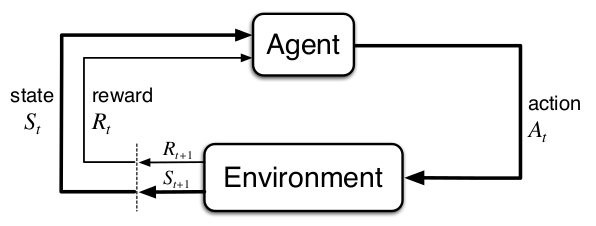
\includegraphics[width=\textwidth]{agent_env_diagram}
    \caption{The agent-environment interaction in MPDs.}
    \label{fig:3.1}
\end{figure}
At each time step $t$ the agent receives a state $s$ and then based on its
policy takes action $a$ on the environment.
Based on this action the agent receives a numerical reward from the env.
With finite MDPs the sets of $\mathcal{S}$, $\mathcal{A}$ and $\mathcal{R}$ are finite.
\begin{myequation}{3.2}
    p(s', r \mid s, a) \doteq Pr \{ S_t=s', R_t=r \mid S_{t-1}=s, A_{t-1}=a\}
\end{myequation}
\begin{myequation}{3.3}
    \sum_{s'}\sum_{r}p(s', r \mid s, a) = 1,
    \forall s \in \mathcal{S}, a \in \mathcal{A}(s)
\end{myequation}
The state must have the \textit{Markov Property} which entails that it holds
all knowledge about the past agent-env interaction that makes a difference
moving forward.
\begin{myequation}{3.4}
    p(s' \mid s,a) \doteq Pr\{S_t = s' \mid S_{t-1} = s, A_{t-1} = a\} =
    \sum_{r} p(s', r \mid s, a)
\end{myequation}
\begin{myequation}{3.5}
    r(s, a) \doteq \mathbb{E}\left[R_t \mid S_{t-1}=s, A_{t-1}=a\right] =
    \sum_{r} r \sum_{s'} p(s', r \mid s, a)
\end{myequation}
\begin{myequation}{3.6}
    r(s, a, s') \doteq
    \mathbb{E}\left[R_t \mid S_{t-1}=s, A_{t-1}=a, S{t}=s'\right] =
    \sum_{r}r \cdot p(s',r \mid s, a)
\end{myequation}

\section{Goals and Rewards}
    The reward signal is your way of communicating to the robot what you want
    it to achieve, not how you want it achieved.

\section{Returns and Episodes}
We define return after step $t$ as
\begin{myequation}{3.7}
    G_t\doteq R_{t+1}+R{t+2}+...+R_T=\sum_{k=0}^{T}R_{t+k+1}
\end{myequation}
\begin{itemize*}
    \item $T$: the terminal state.
    \item $R_t$: reward at time $t$.
\end{itemize*}
We define discounted return for non episodic tasks as:
\begin{myequation}{3.8}
    G_t\doteq \sum_{k=0}^{\infty}\gamma^kR_{t+k+1}
\end{myequation}
\begin{myequation}{3.9}
    G_t\doteq R_{t+1} + \gamma G_{t+1}
\end{myequation}
\begin{itemize*}
    \item $\gamma \in [0, 1]$: the discount rate.
\end{itemize*}
If the reward is a constant +1:
\begin{myequation}{3.10}
    G_t\doteq \sum_{k=0}^{\infty}\gamma^k=\frac{1}{1-\gamma}
\end{myequation}

\section{Unified Notation for Episodic and Continuing Tasks}

\section{Policies and Value Functions}
\textbf{Value functions} show how good a state is, or how good of a move would be to
take an action $a$ at state $s$.
\textbf{Policy} is a mapping from state $s$ to probabilities of taking actions in $A$.

\begin{exercise}{3.11}
    If the current state is $S_t$, and actions are selected
    according to stochastic policy $\pi$, then what is the expectation of $R_{t+1}$
    in terms of $\pi$ and the four-argument function $p$ \hyperref[eq:3.2]{(3.2)}?
    \begin{equation*}
        R_{t+1} = \sum_a \pi(a\mid s)\sum_{s',r}p(s',r\mid a,s)
    \end{equation*}
\end{exercise}

For \hyperref[def:mdp]{MDP}s we define $v_{\pi}$ as the
\textit{state-value function for policy $\pi$}:

\begin{myequation}{3.12}
    \begin{aligned}
        v_{\pi}(s) &\doteq \mathbb{E}_{\pi} \left[G_t \mid S_t = s \right] \\
        &=\mathbb{E}_{\pi}\left[\sum_{k=0}^{\infty}\gamma^k R_{t+k+1} \mid S_t = s\right]
        , \forall s \in \mathcal{S}
    \end{aligned}
\end{myequation}

And $q_{\pi}(s, a)$ as the \textit{action-value function for policy $\pi$}:

\begin{myequation}{3.13}
    \begin{aligned}
        q_{\pi}(s, a) &\doteq \mathbb{E}_{\pi}\left[G_t \mid S_t=s, A_t=a\right] \\
        &=\mathbb{E}_{\pi}\left[\sum_{k=0}^{\infty}\gamma^k R_{t+k+1} \mid S_t=s, A_t=a\right]
    \end{aligned}
\end{myequation}

\begin{exercise}{3.12}
    Give an equation for $v_{\pi}$ in terms of $q_{\pi}$ and $\pi$.
    \begin{equation*}
        v_{\pi} = \sum_a \pi(a\mid s)\cdot q_{\pi}(a, s)
    \end{equation*}
\end{exercise}

\begin{exercise}{3.13}
    Give an equation for $q_{\pi}$ in terms of $v_{\pi}$
    and the four-argument $p$.
    \begin{equation*}
        q_{\pi} = \sum_{s'} v_{\pi}(s') \sum_r p(s',r\mid a,s)
    \end{equation*}
\end{exercise}

\textit{Monte Carlo methods} are RL methods that involve averaging over many random
samples for the actual returns.

\begin{myequation}{3.14}
    \begin{aligned}
        v_{\pi}(s) &\doteq \mathbb{E}_{\pi}\left[G_t \mid S_t=s\right]\\
        &=\mathbb{E}_{\pi}\left[R_{t+1}+\gamma G_{t+1} \mid S_t=s \right] \\
        &=\sum_a \pi(a \mid s) \sum_{s'}\sum_r p(s', r \mid s, a)
        \left[r+\gamma \mathbb{E}_{\pi}\left[G_{t+1}\mid S_{t+1}=s'\right]\right] \\
        &=\sum_a \pi(a \mid s) \sum_{s', r}p(s', r \mid s, a)\left[r+\gamma v_{\pi}(s')\right],
        \forall s \in \mathcal{S}
    \end{aligned}
\end{myequation}

This last equation is the so-called \textit{Bellman equation for $v_{\pi}$} and is essentially
weighing the values in the brackets on the right given the probability \newline
\mbox{$\pi(a\mid s)p(s',r\mid s, a)$}, and iterating through all possibilities.

\begin{figure}[h]
    \centering
    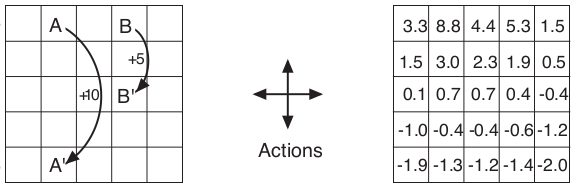
\includegraphics[scale=0.5]{grid_world_ex}
    \caption{Gridworld example: exceptional reward dynamics (left) and state-value function
    for the equiprobable random policy (right).
    Suppose the agent selects all four actions (left, right, up, down) with equal
    probability in all states.
    $\gamma=0.9$.}
    \label{fig:3.2}
\end{figure}

\begin{exercise}{3.17}
    \begin{wrapfigure}{r}{0.3\linewidth}
        \centering
        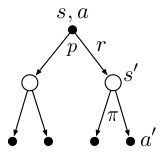
\includegraphics[scale=0.6]{action_value_backup_diagram.png}
    \end{wrapfigure}
    What is the Bellman equation for action values, that is, for $q_{\pi}$?
    It must give the action value $q_{\pi}(s, a)$ in terms of the action
    values, $q_{\pi}(s',a')$, of possible successors to the state-action pair $(s, a)$.
    Hint: The diagram corresponds to this equation.
    Show the sequence of equations analogous to \hyperref[eq:3.14]{(3.14)}, but for action
    values.
    \[
        \begin{aligned}
            q_{\pi}(s,a)
            &=\mathbb{E}_{\pi}\left[\sum_{k=0}^{\infty}\gamma^k R_{t+k+1} \mid S_t=s, A_t=a\right]\\
            &=\sum_{s',r}p(s',r\mid a, s)\cdot r
            + \sum_{s'}p(s'\mid s,a)\cdot\gamma\sum_{a'}\pi (a'|s')\cdot q_{\pi}(s',a')
        \end{aligned}
    \]
\end{exercise}

\begin{exercise}{3.18}
    \begin{center}
        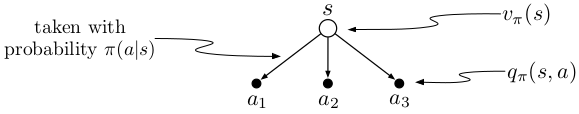
\includegraphics[scale=0.5]{exercise_3_18_diagram}
    \end{center}
    Give the equation corresponding to the root node, $v_{\pi}(s)$, in terms of the
    value at the expected leaf node, $q_{\pi}(s, a)$, given $S_t=s$.
    This equation should include an expectation conditioned on following the policy $\pi$.
    Then give a second equation in which the expected value is written out explicitly
    in terms of $\pi(a|s)$ such that no expected value notation appears in the equation.
    \[
        \begin{aligned}
            v_{\pi}(s)&=\mathbb{E}_{\pi}\left[q_{\pi}(s,a)\right]\\
            &=\sum_{a}\pi(a\mid s)\cdot q_{\pi}(s,a)
        \end{aligned}
    \]
\end{exercise}

\begin{exercise}{3.19}
    \begin{center}
        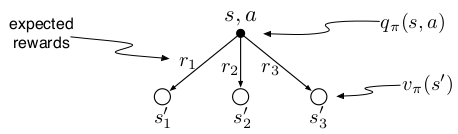
\includegraphics[scale=0.5]{exercise_3_19_diagram}
    \end{center}
    Give the equation corresponding to this intuition and diagram for the action value,
    $q_{\pi}(s,a)$, in terms of the expected new reward, $r_{t+1}$, and the expected
    next state value, $v_{\pi}(s_{t+1})$, given $s_t$ and $a_t$.
    This equation should include an expectation but not one condition on following the policy.
    Then give a second equation, writing out the expected value explicitly in terms of
    $p(s',r\mid s,a)$ defined by \hyperref[eq:3.2]{(3.2)}, such that no expected value notation
    appears in the equation.
    \[
        \begin{aligned}
            q_{\pi}(s,a)&=\mathbb{E}_{s,a}\left[r_{t+1}+\gamma v_{\pi}(s')\right]\\
            &=\sum_{s',r}p(s',r\mid s,a)\cdot r + \gamma\sum_{s'}p(s'\mid s,a)\cdot v_{\pi}(s')
        \end{aligned}
    \]
\end{exercise}

\section{Optimal Policies and Optimal Value Functions}
A policy $\pi'$ is better than policy $\pi$ if $\forall s \in \mathcal{S}, v_{\pi'}\geq v_{\pi}$.
In other words
\[
    \pi'\geq \pi \Longleftrightarrow (\forall s\in\mathcal{S})(v_{\pi'}\geq v_{\pi})
\]

\textit{Optimal policy}:
\begin{myequation}{3.60*}
    \pi_*\doteq \max_{v_{\pi}(s)}\pi,\forall s\in\mathcal{S}
\end{myequation}
\textit{Optimal state-value function}:
\begin{myequation}{3.15}
    v_*(s)\doteq \max_{\pi}v_{\pi}(s),\forall s\in\mathcal{S}
\end{myequation}
\textit{Optimal action-value function}:
\begin{myequation}{3.16}
    q_*(s,a)\doteq \max_{\pi}q_{\pi}(a,s),\forall s\in\mathcal{S},\forall a\in\mathcal{A}
\end{myequation}
\begin{myequation}{3.17}
    q_*(s,a)=\mathbb{E}\left[R_{t+1}+\gamma v_*(S_{t+1})\in S_t=s,A_t=a\right]
\end{myequation}
\textit{Bellman optimality equation}:
\begin{myequation}{3.18}
    \begin{aligned}
        v_*(s)&=\max_{a\in\mathcal{A}(s)}q_{\pi_*}(s,a)\\
        &=\max_a\mathbb{E}_{\pi_*}\left[G_t\mid S_t=s,A_t=a\right]\\
        &=\max_a\mathbb{E}\left[R_{t+1}+\gamma v_*(S_{t+1})\mid S_t=s,A_t=a\right]\\
        &=\max_a\sum_{s',r}p(s',r\mid s,a)[r+\gamma v_*(s')]
    \end{aligned}
\end{myequation}
\begin{myequation}{3.20}
    \begin{aligned}
        q_*(s,a)&=\mathbb{E}\left[
            R_{t+1}+\gamma\max_{a'}q_*(S_{t+1},a')\mid S_t=s,A_t=a
        \right]\\
        &=\sum_{s',r}p(s',r\mid s,a)\left[r+\gamma\max_{a'}q_*(s',a')\right]
    \end{aligned}
\end{myequation}

Solving the \textit{Bellman optimality equations} relies on having having the following three
properties that are rarely found in real-world scenarios:
\begin{itemize}
    \item accurate knowledge of the dynamics of the environment.
    \item computational resources to complete the computation of the solution.
    \item the Markov property.
\end{itemize}

\begin{exercise}{3.25}
    Give an equation for $v_*$ in terms of $q_*$.
    \[
        v_*(s) = \max_a q_*(s,a)
    \]
\end{exercise}
\begin{exercise}{3.26}
    Give an equation for $q_*$ in terms of $v_*$ and the four-argument
    $p$ \hyperref[eq:3.2]{(3.2)}.
    \[
        q_*(s, a) = \sum_{s',r}p(s',r\mid s,a)\cdot(r + \gamma v_*(s'))
    \]
\end{exercise}
\begin{exercise}{3.29 !?}
    Rewrite the four Bellman equations for the four value functions
    ($v_{\pi}, v_*, q_{\pi}, q_*$) in terms of the three-argument
    function $p$ \hyperref[eq:3.4]{(3.4)} and the two-argument
    function $r$ \hyperref[eq:3.5]{(3.5)}.
    \[
        \begin{aligned}
            v_{\pi}(s)&=\sum_a\pi(a\mid s)
            \sum_{s', r}p(s',r\mid s,a)\left[r+\gamma v_{\pi}(s')\right] \\
            &=\sum_a\pi(a\mid s)\cdot r(s,a)\cdot\gamma
            \sum_{s'}p(s'\mid s,a)]\cdot v_{\pi}(s') \\
        \end{aligned}
    \]
\end{exercise}

\section{Optimality and Approximation}
Tabular methods can store the optimal policy in a table but a lot of RL problems have
a huge number of states that cannot be represented through a table due to memory restrictions.
Therefore, we resolve to approximation methods.


\section{Summary}
\label{sec:fmdps-summary}
Let us summarize the elements of the reinforcement learning problem that we have
presented in this chapter. Reinforcement learning is about learning from interaction
how to behave in order to achieve a goal. The reinforcement learning agent and its
environment interact over a sequence of discrete time steps. The specification of their
interface defines a particular task: the actions are the choices made by the agent; the
states are the basis for making the choices; and the rewards are the basis for evaluating
the choices. Everything inside the agent is completely known and controllable by the
agent; everything outside is incompletely controllable but may or may not be completely
known. A policy is a stochastic rule by which the agent selects actions as a function of
states. The agent’s objective is to maximize the amount of reward it receives over time.
When the reinforcement learning setup described above is formulated with well defined
transition probabilities it constitutes a Markov decision process (MDP). A finite MDP is
an MDP with finite state, action, and (as we formulate it here) reward sets. Much of the
current theory of reinforcement learning is restricted to finite MDPs, but the methods
and ideas apply more generally.
The return is the function of future rewards that the agent seeks to maximize (in
expected value). It has several different definitions depending upon the nature of the
task and whether one wishes to discount delayed reward. The undiscounted formulation
is appropriate for episodic tasks, in which the agent–environment interaction breaks
naturally into episodes; the discounted formulation is appropriate for continuing tasks, in
which the interaction does not naturally break into episodes but continues without limit.
We try to define the returns for the two kinds of tasks such that one set of equations can
apply to both the episodic and continuing cases.
A policy’s value functions assign to each state, or state–action pair, the expected return
from that state, or state–action pair, given that the agent uses the policy. The optimal
value functions assign to each state, or state–action pair, the largest expected return
achievable by any policy. A policy whose value functions are optimal is an optimal policy.
Whereas the optimal value functions for states and state–action pairs are unique for a
given MDP, there can be many optimal policies. Any policy that is greedy with respect to
the optimal value functions must be an optimal policy. The Bellman optimality equations
are special consistency conditions that the optimal value functions must satisfy and that
can, in principle, be solved for the optimal value functions, from which an optimal policy
can be determined with relative ease.
A reinforcement learning problem can be posed in a variety of different ways depending
on assumptions about the level of knowledge initially available to the agent. In problems
of complete knowledge, the agent has a complete and accurate model of the environment’s
dynamics. If the environment is an MDP, then such a model consists of the complete four-
argument dynamics function $p$ (\ref{eq:3.2}).
In problems of incomplete knowledge, a complete
and perfect model of the environment is not available.
Even if the agent has a complete and accurate environment model, the agent is
typically unable to perform enough computation per time step to fully use it. The
memory available is also an important constraint. Memory may be required to build
up accurate approximations of value functions, policies, and models. In most cases of
practical interest there are far more states than could possibly be entries in a table, and
approximations must be made.
A well-defined notion of optimality organizes the approach to learning we describe in
this book and provides a way to understand the theoretical properties of various learning
algorithms, but it is an ideal that reinforcement learning agents can only approximate
to varying degrees. In reinforcement learning we are very much concerned with cases in
which optimal solutions cannot be found but must be approximated in some way.


\chapter{Dynamic Programming}
\label{ch:dp}
DP algorithms are obtained by turning the Bellman equations into assignments - update rules
for improving approximations in the future.

\section{Policy Evaluation (Prediction)}
\label{sec:policy_evaluation}
\emph{Policy evaluation} is the process of determining
$v_{\pi}(s), \forall s\in\mathcal{S}$.
\emph{Iterative policy evaluation} is the process of arbitrarily initializing the state-value
function for all states and then using the Bellman equation as an iterative update rule.
\begin{center}
    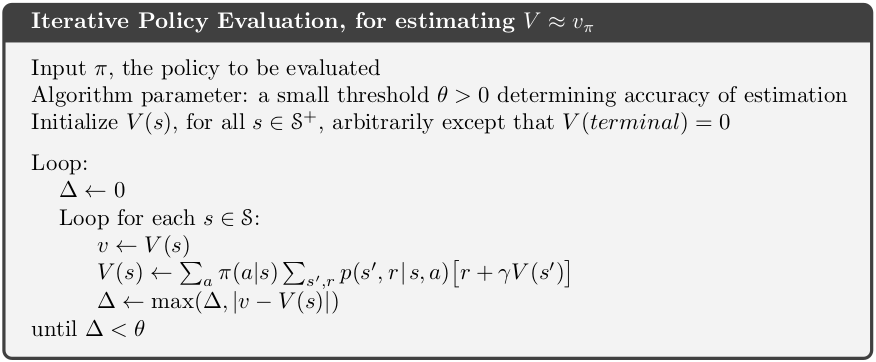
\includegraphics[width=\textwidth]{img/alg_iterative_policy_eval.png}
\end{center}

\section{Policy Improvement}
\label{sec:policy_improvement}
If we find policy $\pi'$ such that $q_{\pi'}(s,\pi'(s))\geq v_{\pi}(s)$ then we update
the policy $\pi$ so that $\pi(s)==\pi'(s)$.
At each step we select the action that appears best according to $q_{\pi}(s,a)$, the new
\textit{greedy} policy $\pi'$ is defined as the following:
\begin{myequation}{4.9}
    \begin{aligned}
        \pi'(s)&\doteq \argmax_a q_{\pi}(s,a) \\
        &=\argmax_a\sum_{s',r}p(s',r\mid s,a)\left[r+\gamma v_{\pi}(s')\right]
    \end{aligned}
\end{myequation}
\begin{itemize*}
    \item $\argmax_a$: value of $a$ for which the expression that follows is maximized.
\end{itemize*}
\emph{Policy improvement} is the process of making a new policy
that improves the original policy by making it greedy with respect to the value function of
the original policy.

\section{Policy Iteration}
\begin{center}
    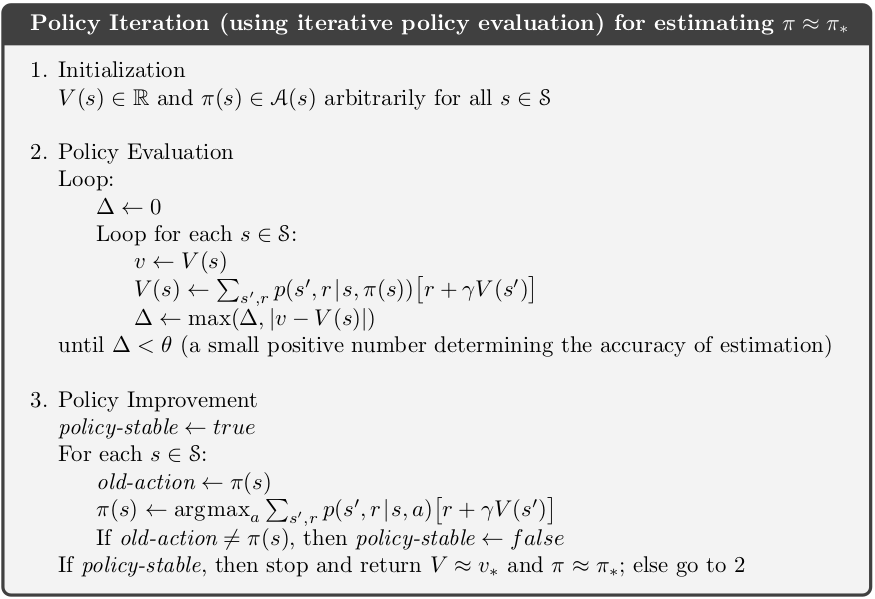
\includegraphics[width=\textwidth]{img/alg_iterative_policy_improvement.png}
\end{center}

\section{Value Iteration}
We are truncating \myref{sec:policy_evaluation}{policy evaluation} to get faster computation
but still ensure convergence.
Value iteration is truncating \myref{sec:policy_evaluation}{policy evaluation} to exactly one step.

\begin{myequation}{4.10}
    \begin{aligned}
        v_{k+1}(s)&\doteq\max_a\mathbb{E}\left[R_{t+1} + \gamma v_k(S_{t+1})\mid S_t=s,A_t=a\right] \\
        &=\max_a\sum_{s',r}p(s',r\mid s,a)\left[r+\gamma v_k(s')\right]
    \end{aligned}
\end{myequation}
\begin{center}
    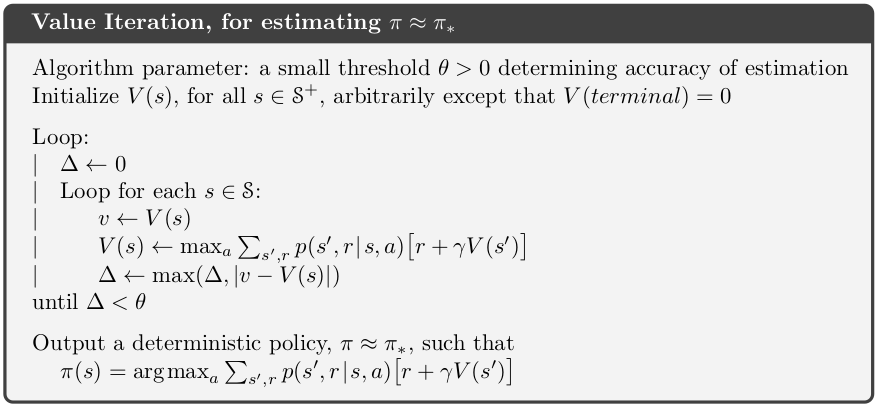
\includegraphics[width=\textwidth]{img/alg_value_iteration.png}
\end{center}

\section{Asynchronous Dynamic Programming}
These algorithms don't update all state values in each sweep but only target some.
This targeting can be done using the amount of update done in a sweep on a state, or given
preset priorities.
They also allow for real-time interaction - while an agent is playing the algorithm is running and learning.

\section{Generalized Policy Iteration (GPI)}
\label{sec:gpi}
\textit{Generalized Policy Iteration} (GPI) refers to a branch of algorithms
that allow for \myref{sec:policy_evaluation}{policy evaluation} and
\myref{sec:policy_improvement}{policy improvement} to intertwine.
\begin{center}
    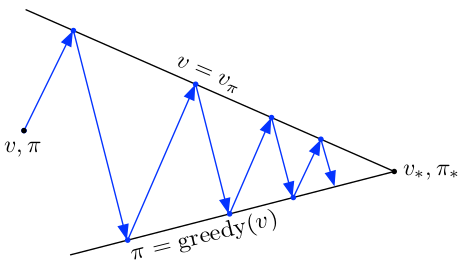
\includegraphics[scale=0.43]{img/general_policy_iteration_diagram.png}
\end{center}

\section{Efficiency of Dynamic Programming}

\section{Summary}
In this chapter we have become familiar with the basic ideas and algorithms of dynamic
programming as they relate to solving finite MDPs. Policy evaluation refers to the (typi-
cally) iterative computation of the value functions for a given policy. Policy improvement
refers to the computation of an improved policy given the value function for that policy.
Putting these two computations together, we obtain policy iteration and value iteration,
the two most popular DP methods. Either of these can be used to reliably compute
optimal policies and value functions for finite MDPs given complete knowledge of the
MDP.
Classical DP methods operate in sweeps through the state set, performing an expected
update operation on each state. Each such operation updates the value of one state
based on the values of all possible successor states and their probabilities of occurring.
Expected updates are closely related to Bellman equations: they are little more than
these equations turned into assignment statements. When the updates no longer result in
any changes in value, convergence has occurred to values that satisfy the corresponding
Bellman equation. Just as there are four primary value functions (v ⇡ , v ⇤ , q ⇡ , and q ⇤ ),
there are four corresponding Bellman equations and four corresponding expected updates.
An intuitive view of the operation of DP updates is given by their backup diagrams.
Insight into DP methods and, in fact, into almost all reinforcement learning methods,
can be gained by viewing them as generalized policy iteration (GPI). GPI is the general idea
of two interacting processes revolving around an approximate policy and an approximate
value function. One process takes the policy as given and performs some form of policy
evaluation, changing the value function to be more like the true value function for the
policy. The other process takes the value function as given and performs some form
of policy improvement, changing the policy to make it better, assuming that the value
function is its value function. Although each process changes the basis for the other,
overall they work together to find a joint solution: a policy and value function that are
unchanged by either process and, consequently, are optimal. In some cases, GPI can be
proved to converge, most notably for the classical DP methods that we have presented in
this chapter. In other cases convergence has not been proved, but still the idea of GPI
improves our understanding of the methods.
It is not necessary to perform DP methods in complete sweeps through the state
set. Asynchronous DP methods are in-place iterative methods that update states in an
arbitrary order, perhaps stochastically determined and using out-of-date information.
Many of these methods can be viewed as fine-grained forms of GPI.
Finally, we note one last special property of DP methods. All of them update estimates
of the values of states based on estimates of the values of successor states. That is, they
update estimates on the basis of other estimates. We call this general idea bootstrapping.
Many reinforcement learning methods perform bootstrapping, even those that do not
require, as DP requires, a complete and accurate model of the environment. In the next
chapter we explore reinforcement learning methods that do not require a model and do
not bootstrap. In the chapter after that we explore methods that do not require a model
but do bootstrap. These key features and properties are separable, yet can be mixed in
interesting combinations.


\chapter{Monte Carlo (MC) Methods}
\label{ch:mcm}
Unlike the previous chapters here we only require experience, and not a complete knowledge of the env.
The term \textit{Monte Carlo} is often used in a more broad sense for any estimation method that
invlolves a significant random component.
We are learning the value function based on the sample returns from the MDP.
The idea of gaining experience and averaging returns from each state to estimate the value functions
is an essential idea of all MC methods.
In comparison to DP algorithms, that are breadth-first we can view MCMs as depth-first
algorithms.
MCMs do not bootstrap - an estimation of the value of one state is not based on estimations
of value functions for other states.

\section{Monte Carlo Prediction}
\textit{First-visit MC methods} average returns following the first visit to state $s$.
\textit{Every-visit MC methods} average returns following every visit to state $s$.
\begin{center}
    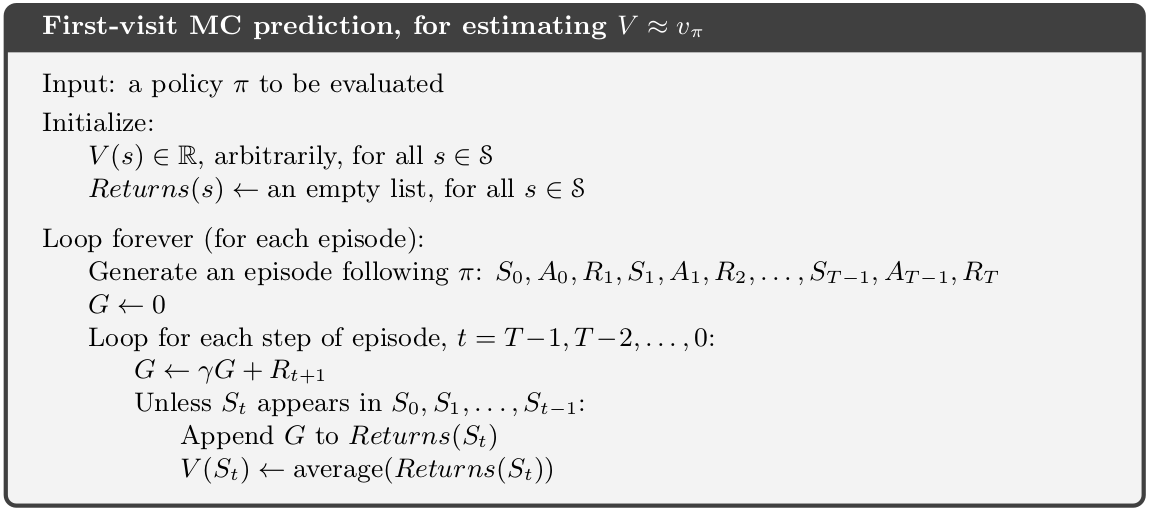
\includegraphics[width=\textwidth]{img/first_visit_MCM.png}
\end{center}

\section{Monte Carlo Estimation of Action Values}
The problem of lack of exploration.
Possible solution with exploring starts, even though this can be used only under specific
circumstances.

\section{Monte Carlo Control}
\begin{center}
    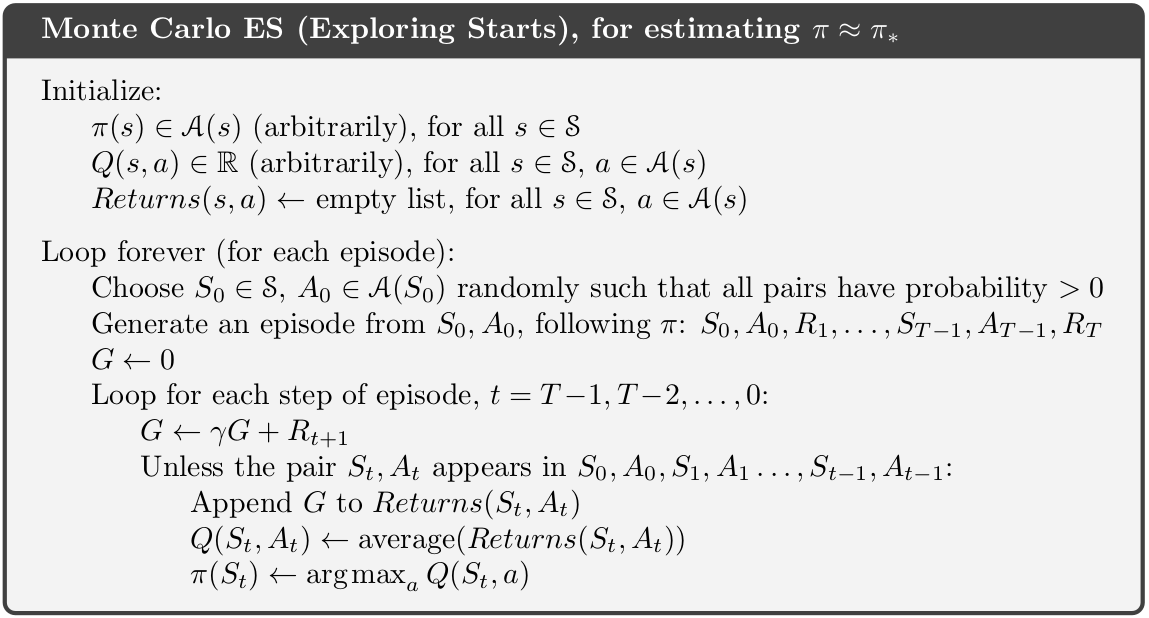
\includegraphics[width=\textwidth]{img/alg_MCM_ES.png}
\end{center}
We can modify the algorithm to only store the mean and the count in $Returns$, rather than the whole list
of returns.
This way we optimize in memory consumption and remove the time needed to calculate the average when
storing $Q(S_t, A_t)$.

\section{Monte Carlo Control without Exploring Starts}
\emph{On-policy methods}\label{t:on_policy_methods} evaluate or improve the policy used to
make decisions, whereas \emph{off-policy methods}\label{t:off_policy_methods} evaluate or
improve a policy different from the one used to make decisions.
\begin{center}
    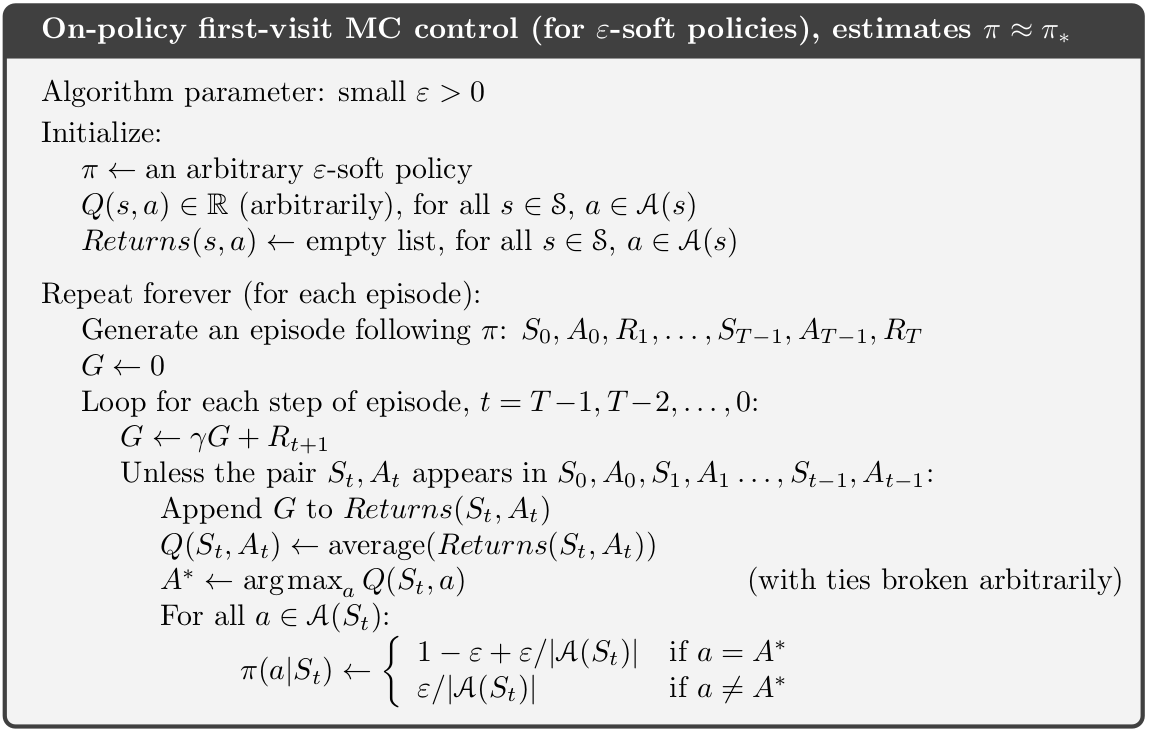
\includegraphics[width=\textwidth]{img/alg_on_policy_first_visit_MC_control.png}
\end{center}

\section{Off-policy Prediction via Importance\newline Sampling}
\label{sec:off_policy_prediction_via_importance_sampling}
Learn the optimal policy while behaving according to an exploratory policy.
The policy being learned about is the \textit{target policy}, and the policy used to generate
behavior is called the \textit{behavior policy}.
\textit{Off-policy} methods are usually of greater variance and slower to converge.
If $b$ is the behavior policy and $\pi$ the target policy then
$\pi(a\mid s)>0\rightarrow b(a\mid s)>0$ - this is called the assumption of \textit{coverage}.
Meaning that every state, action for which $\pi$ has a non-zero value (covers it), policy
$b$ also has a non-zero value, and technically will eventually cover it too.
\newline\emph{Importance sampling ratio}\label{t:importance_sampling_ratio} given a
state-action trajectory:
\begin{myequation}{5.3}
    \rho_{t:T-1}\doteq \prod_{k=t}^{T-1}\frac{\pi(A_k\mid S_k)}{b(A_k\mid S_k)}
\end{myequation}
We use the importance sampling ratio to transform the estimated $v_b(s)$ to $v_\pi(s)$:
\begin{myequation}{5.4}
    v_{\pi}(s) = \mathbb{E}\left[\rho_{t:T-1}\cdot G_t\mid S=s\right]
\end{myequation}
Here the timesteps will surpass episode boundaries.
If we define $\mathcal{T}(s)$ as a set of all time steps where $s$ was encountered;
only the first times per episode for first-visit methods.
Let $T(t)$ denote the first time of termination after $t$, and $G_t$ denote the return after $t$ following
up to $T(t)$, then we can estimate $v_\pi(s)$ as:
\begin{myequation}{5.5}
    V(s)\doteq\frac{\sum_{t\in\mathcal{T}(s)}\rho_{t:T(t)-1}G_t}{|\mathcal{T}(s)|}
\end{myequation}
When \emph{importance sampling} is done as a simple average in this way it's called
\emph{ordinary importance sampling}\label{t:ordinary_importance_sampling}.
An important alternative to that is
\emph{weighted importance sampling}\label{t:weighted_importance_sampling} that uses
weighted averages:
\begin{myequation}{5.6}
    V(s)\doteq\frac{\sum_{t\in\mathcal{T}(s)}\rho_{t:T(t)-1}G_t}
    {\sum_{t\in\mathcal{T}(s)}\rho_{t:T(t)-1}}
\end{myequation}

\section{Incremental Implementation}
\begin{center}
    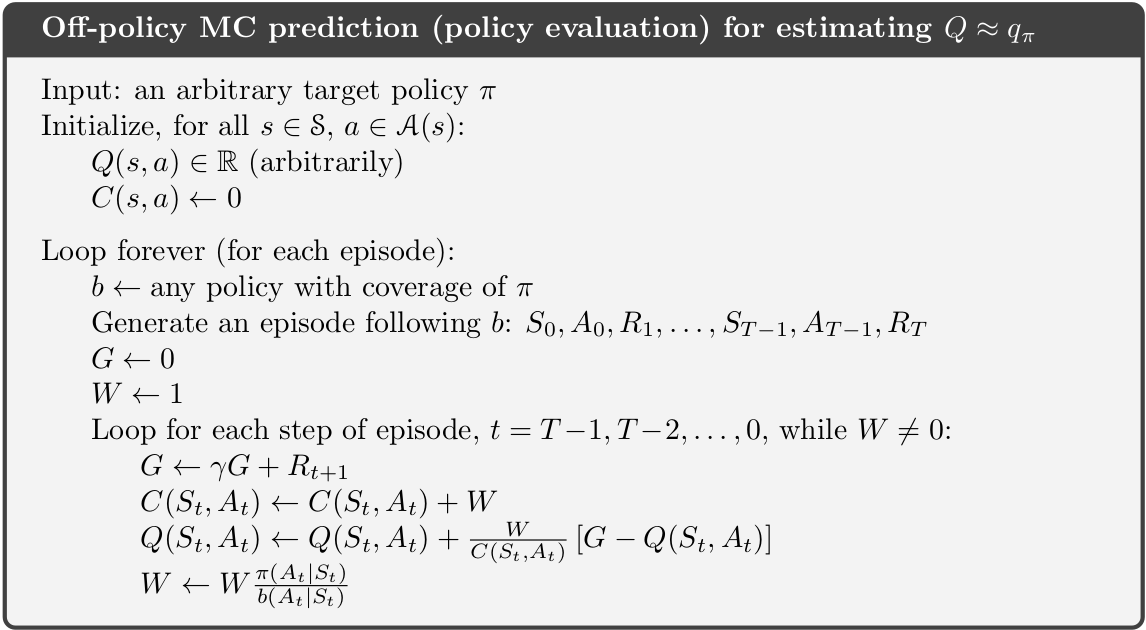
\includegraphics[width=\textwidth]{img/alg_off_policy_mc_prediction.png}
    \begin{itemize*}
        \item $C(s,a)$: cumulative sum of the weights.
    \end{itemize*}
\end{center}

\section{Off-policy Monte Carlo Control}
\begin{center}
    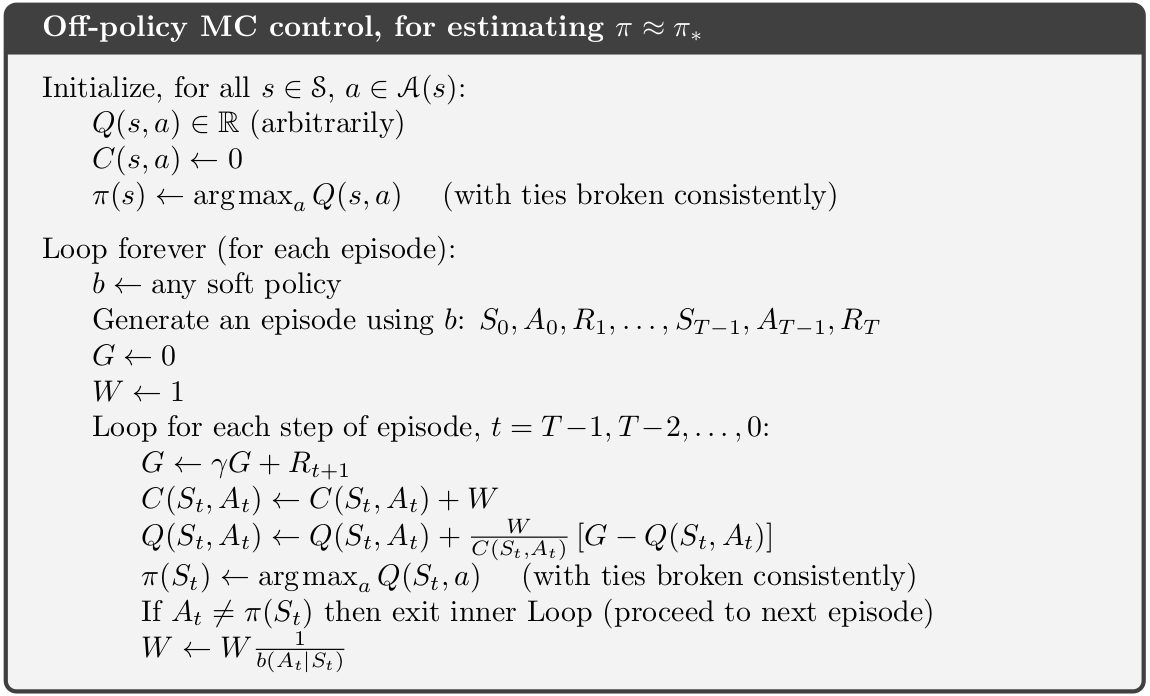
\includegraphics[width=\textwidth]{img/alg_off_policy_mc_control.png}
\end{center}

\section{*Discounting-aware Importance Sampling}
\emph{Importance sampling} ($\rho$) takes into account all timesteps leading up to $T$.
What it should preferably be doing is looking at the discount to $G$ which is $\gamma$ and
using that to discount the $\rho$.
We can look into $\gamma$ as partially terminating $G$ and then define
\emph{flat partial returns} ($\bar{G}_{t:h}$) as:

\begin{equation*}
    \bar{G} \doteq R_{t+1} + R_{t+2} + \cdots + R_h,
    \hspace{3em}
    0 \leq t \le h \leq T
\end{equation*}

They're called \emph{flat} because there's no discounting, and \emph{partial} because rather
than going to $T$ they end at $h$, called the \emph{horizon}.

\begin{equation*}
    G_t \doteq (1-\gamma)\sum_{h=t+1}^{T-1}\gamma^{h-t-1}\bar{G}_{t:h}
        + \gamma^{T-t-1}\bar{G}_{t:T}
\end{equation*}

Given this, (\ref{eq:5.5}) and (\ref{eq:5.6}) become discount aware importance
sampling estimators:

\begin{myequation}{5.9}
    V(s)\doteq\frac{
        \sum_{t\in\mathcal{T}(s)}\left(
            (1-\gamma)\sum_{h=t+1}^{T(t)-1}\gamma^{h-t-1}\rho_{t:h-1}\bar{G}_{t:h}+
            \gamma^{T(t)-t-1}\rho_{t:T(t)-1}\bar{G}_{t:T(t)}
        \right)
    }{|\mathcal{T}(s)|}
\end{myequation}

\begin{myequation}{5.10}
    V(s)\doteq\frac{
        \sum_{t\in\mathcal{T}(s)}\left(
            (1-\gamma)\sum_{h=t+1}^{T(t)-1}\gamma^{h-t-1}\rho_{t:h-1}\bar{G}_{t:h}+
            \gamma^{T(t)-t-1}\rho_{t:T(t)-1}\bar{G}_{t:T(t)}
        \right)
    }{
        \sum_{t\in\mathcal{T}(s)}\left(
            (1-\gamma)\sum_{h=t+1}^{T(t)-1}\gamma^{h-t-1}\rho_{t:h-1}+
            \gamma^{T(t)-t-1}\rho_{t:T(t)-1}
        \right)
    }
\end{myequation}

\section{*Per-decision Importance Sampling}
\label{sec:per_decision_importance_sampling}
To further minimize the variance, we can multiply a given $R$ at time $t$ with just the
$\rho_{t0:t-1}$ because those after do not influence the reward.

\begin{equation*}
    \begin{gathered}
        \mathbb{E}\left[\rho_{t:T-1}R_{t+k}\right]=\mathbb{E}\left[\rho_{t:t-k-1}R_{t+k}\right]
        \Rightarrow
        \mathbb{E}\left[\rho_{t:T-1}G_t\right]=\mathbb{E}\left[\tilde{G}_t\right] \\
        \tilde{G}_t=\rho_{t:t}R_{t+1}+\gamma\rho_{t:t+1}R_{t+2}+\cdots
        +\gamma^{k-1}\rho_{t:t+k-1}R_{t+k}+\cdots+\gamma^{T-1}\rho_{t:T-1}R_T\\
    \end{gathered}
\end{equation*}

Now (\ref{eq:5.5}) becomes:

\begin{myequation}{5.15}
    V(s)=\frac{\sum_{t\in\mathcal{T}(s)}\tilde{G}_t}{|\mathcal{T}(s)|}
\end{myequation}

\section{Summary}
The Monte Carlo methods presented in this chapter learn value functions and optimal
policies from experience in the form of sample episodes.
This gives them at least three kinds of advantages over DP methods.
\begin{enumerate}
    \item They can be used to learn optimal behavior directly from interaction with the
    environment, with no model of the environment’s dynamics.
    \item They can be used with simulation or sample models.
    For surprisingly many applications it is easy to simulate sample episodes even though
    it is difficult to construct the kind of explicit model of transition probabilities
    required by DP methods.
    \item It is easy and efficient to focus Monte Carlo methods on a small subset of the states.
    A region of special interest can be accurately evaluated without going to the expense of
    accurately evaluating the rest of the state set (we explore this further in Chapter 8).
    \item They may be less harmed by violations of the Markov property.
    This is because they do not update their value estimates on the basis of the value
    estimates of successor states.
    In other words, it is because they do not bootstrap.
\end{enumerate}

In designing Monte Carlo control methods we have followed the overall schema of
\myref{sec:gpi}{GPI} introduced in Chapter 4.
\myref{sec:gpi}{GPI} involves interacting processes of
\myref{sec:policy_evaluation}{policy evaluation} and
\myref{sec:policy_improvement}{policy improvement}.
Monte Carlo methods provide an alternative \myref{sec:policy_evaluation}{policy evaluation}
process.
Rather than use a model to compute the value of each state, they simply average many returns
that start in the state.
Because a state’s value is the expected return, this average can become a good approximation
to the value.
In control methods we are particularly interested in approximating action-value functions,
because these can be used to improve the policy without requiring a model of the
environment’s transition dynamics.
Monte Carlo methods intermix policy evaluation and policy improvement steps on an
episode-by-episode basis, and can be incrementally implemented on an episode-by-episode basis.
Maintaining sufficient exploration is an issue in Monte Carlo control methods.
It is not enough just to select the actions currently estimated to be best, because then no
returns will be obtained for alternative actions, and it may never be learned that they
are actually better.
One approach is to ignore this problem by assuming that episodes begin with state–action pairs
randomly selected to cover all possibilities.
Such \emph{exploring starts} can sometimes be arranged in applications with simulated episodes,
but are unlikely in learning from real experience.
In \myref{t:on_policy_methods}{on-policy methods}, the agent commits to always exploring and tries to find the
best policy that still explores.
In \myref{t:off_policy_methods}{off-policy methods}, the agent also explores, but learns a deterministic optimal policy that
may be unrelated to the policy followed.
\emph{Off-policy prediction} refers to learning the value function of a target policy from data
generated by a different behavior policy.
Such learning methods are based on some form of
\myref{sec:off_policy_prediction_via_importance_sampling}{importance sampling}, that is,
on weighting returns by the ratio of the probabilities of taking the observed actions under
the two policies, thereby transforming their expectations from the behavior policy to the
target policy.
\myref{t:ordinary_importance_sampling}{Ordinary importance sampling} uses a simple average of
the weighted returns, whereas
\myref{t:weighted_importance_sampling}{weighted importance sampling} uses a weighted average.
Ordinary importance sampling produces unbiased estimates, but has larger, possibly infinite,
variance, whereas weighted importance sampling always has finite variance and is preferred in
practice.
Despite their conceptual simplicity, \myref{t:off_policy_methods}{off-policy}
Monte Carlo methods for both prediction and control remain unsettled and are a subject
of ongoing research.
The Monte Carlo methods treated in this chapter differ from the DP methods treated
in the previous chapter in two major ways.
\begin{enumerate}
    \item They operate on sample experience, and thus can be used for direct learning
    without a model.
    \item They do not bootstrap.
    That is, they do not update their value estimates on the basis of other value estimates.
\end{enumerate}
These two differences are not tightly linked, and can be separated.
In the next chapter we consider methods that learn from experience, like Monte Carlo methods,
but also bootstrap, like DP methods.


\chapter{Temporal-Difference Learning}
\label{ch:temporal_difference_learning}
\emph{Temporal-difference learning} is a combination of \myref{ch:mcm}{MC}
and \myref{ch:dp}{DP} methods, it generates experience from which it learns, like \emph{MC},
and it bootstraps like \emph{DP}.

\section{TD Prediction}
\label{sec:td_prediction}
Similar to how \emph{MC} methdods predict but we stop right after the first step and then
use the approximated value.
Basically, the target is $R_{t+1}+\gamma V(S_{t+1})$ instead of $G_t$.

\begin{myequation}{6.2}
    V(S_t)\leftarrow V(S_t) + \alpha\left[R_{t+1}+\gamma V(S_{t+1})-V(S_t)\right]
\end{myequation}

This is called $TD(0)$ or \emph{one-step TD}\label{t:tdl-one_step_td}.

\begin{center}
    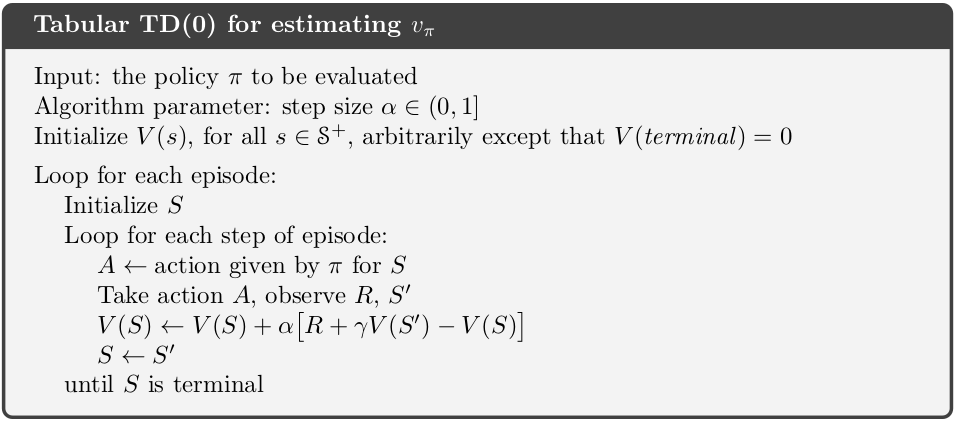
\includegraphics[width=\textwidth]{img/td0.png}
\end{center}

We can notice that the value in the brackets in (\ref{eq:6.2}) is a sort of error.
That error is called \emph{TD error} ($\delta$)\label{t:td_error} and it is the
difference from the estimated value of $S_t$ and the better estimate after the next step
$R_{t+1}+\gamma V(S_{t+1})$.

\begin{myequation}{6.5}
    \delta_t\doteq R_{t+1}+\gamma V(S_{t+1})-V(S_t)
\end{myequation}

\section{Advantages of TD Prediction Methods}
\label{sec:advantages_of_td_prediction_methods}

\section{Optimality of TD(0)}
\label{sec:optimality_of_td0}
Consider an example where we use \emph{batch updating}.
\myref{ch:temporal_difference_learning}{TD(0)} and constant $\alpha$ \myref{ch:mcm}{MCM}
converge to different values.
Observe the following episodes:
\begin{wrapfigure}{r}{0.4\linewidth}
    \centering
    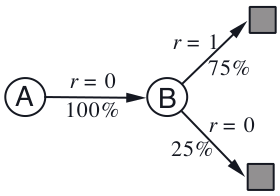
\includegraphics[scale=0.4]{img/ex6_4.png}
\end{wrapfigure}
\begin{multicols}{2}
    \begin{enumerate}
        \item $A,0,B,0$
        \item $B,1$
        \item $B,1$
        \item $B,1$
        \item $B,1$
        \item $B,1$
        \item $B,1$
        \item $B,0$
    \end{enumerate}
\end{multicols}

Both batch TD(0) and batch MC would conclude that $V(B)=\frac{3}{4}$ but TD(0) would
approximate $V(A)=V(B)=\frac{3}{4}$ whereas MC would approximate $V(A)=0$ because the one
episode we go through the state we get reward $0$.

Batch MC methods always find the estimates that minimize mean-squared error on the
training set, whereas batch TD(0) always finds the estimates that would be exactly correct
for the maximum-likelihood model of the Markov process.
In general, the \emph{maximum-likelihood estimate} of a parameter is the parameter value
whose probability of generating the data is greatest.
In this case, the maximum-likelihood estimate is the model of the Markov process formed in the
obvious way from the observed episodes: the estimated transition probability from $i$ to $j$
is the fraction of observed transitions from $i$ that went to $j$, and the associated expected
reward is the average of the rewards observed on those transitions.
Given this model, we can compute the estimate of the value function that would be exactly
correct if the model were exactly correct.
This is called the \emph{certainty-equivalence estimate} because it is equivalent to assuming
that the estimate of the underlying process was known with certainty rather than being
approximated.

\section{Sarsa: On-policy TD Control}
\label{sec:sarsa_on_policy_td_control}
Instead of state values we use action values:
\begin{myequation}{6.7}
    \delta_t\doteq R_{t+1}+\gamma Q(S_{t+1},A_{t+1})-Q(S_t,A_t) \\
    Q(S_t,A_t)\leftarrow Q(S_t,A_t)+\alpha\cdot\delta_t
\end{myequation}

\begin{center}
    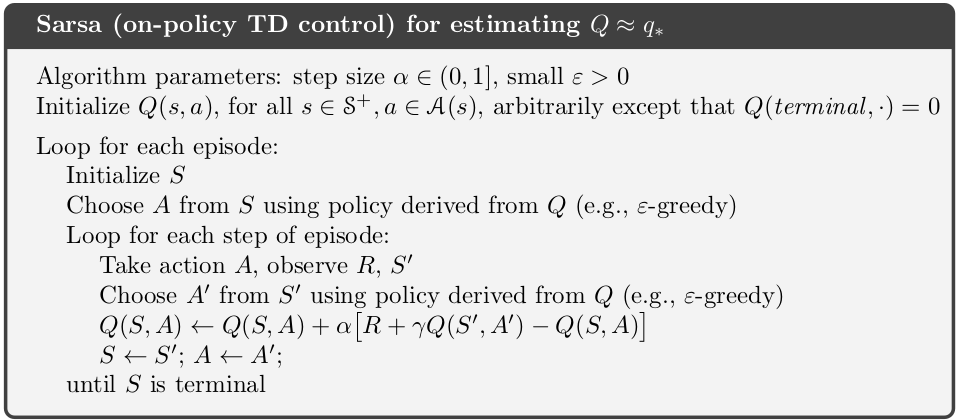
\includegraphics[width=\textwidth]{img/alg_sarsa.png}
\end{center}

\section{Q-Learning: Off-policy TD Control}
\label{sec:q_learning_off_policy_td_control}
Instead of using $Q(S_{t+1}, A{t+1})$ for action $A_{t+1}$ taken by the \emph{behavior policy} we
use $\max_aQ(S_{t+1}, a)$.

\begin{myequation}{6.8}
    \delta_t\doteq R_{t+1}+\max_aQ(S_{t+1},a)-Q(S_t,A_t) \\
    Q(S_t,A_t)\leftarrow Q(S_t,A_t)+\alpha\cdot\delta_t
\end{myequation}

All that is required for correct convergence is that all pairs continue to be updated.

\begin{center}
    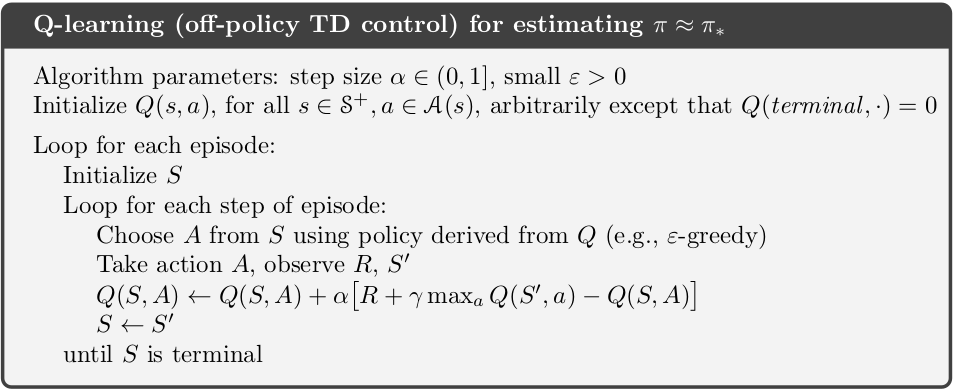
\includegraphics[width=\textwidth]{img/alg_q_learning.png}
\end{center}

\section{Expected SARSA}
\label{sec:expected_sarsa}

\begin{myequation}{6.9}
    \begin{aligned}
        \delta_t
        &\doteq R_{t+1}+\gamma\mathbb{E}\left[Q(S_{t+1},A_{t+1}\mid S_{t+1})\right]-Q(S_t,A_t)\\
        &\doteq R_{t+1}+\gamma\sum_a\pi(a\mid S_{t+1})Q(S_{t+1},a)-Q(S_t,A_t)
    \end{aligned} \\
    Q(S_t,A_t)\leftarrow Q(S_t,A_t)+\alpha\cdot\delta_t
\end{myequation}

\section{Maximization Bias and Double Learning}
\label{sec:maximization_bias_and_double_learning}
A maximum over estimated values is used implicitly as an estimate of the maximum value, which can
lead to a significant positive bias.
To see why, consider a single state s where there are many actions a whose true values,
$q(s,a)$, are all zero but whose estimated values, $Q(s,a)$, are uncertain and thus distributed
some above and some below zero.
The maximum of the true values is zero, but the maximum of the estimates
is positive, a positive bias.
We call this \emph{maximization bias}\label{t:maximization_bias}.

The reason this bias occurs is because we are using the same state-action value function to
approximate $q(s,a)$ and then using the maximum of the estimation of $q(s,a)$ to estimate the
maximum of $q(s,a)$ - the optimal action.
To attempt and mitigate this issue, we can learn two independent estimates of the state-action
value ($Q_1, Q_2$) and then using them generate an unbiased estimate of the maximum of $q(s,a)$.
We get the optimal action from one of the estimates to update the other.
\begin{myequation}{6.10}
    \delta_t\doteq R_{t+1}+\gamma Q_1(S_t,\argmax_aQ_2(S_{t+1},a))-Q_1(S_t,A_t) \\
    Q_1(S_t,A_t)\leftarrow Q_1(S_t,A_t)+\alpha\delta_t
\end{myequation}

\begin{center}
    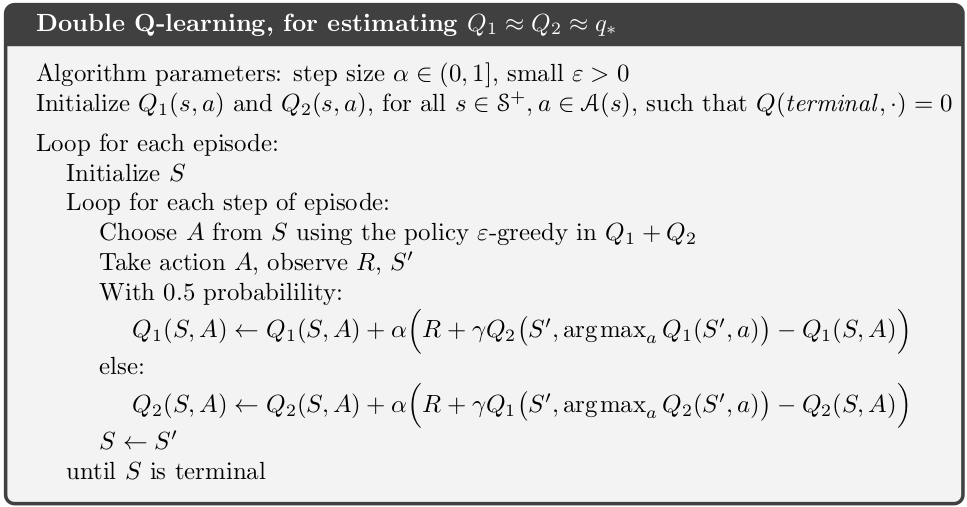
\includegraphics[width=\textwidth]{img/alg_dq_learning.png}
\end{center}

\section{Games, Afterstates, and Other Special Cases}
\label{sec:games_afterstates_and_other_special_cases}
A conventional state-value function evaluates states in which the agent has the option of
selecting an action, but the state-value function used in tic-tac-toe evaluates board positions
after the agent has made its move.
Let us call these \emph{afterstates}\label{t:afterstate}, and value functions over these,
\emph{afterstate value functions}\label{t:afterstate_value_functions}.

\begin{figure}[h]
    \centering
    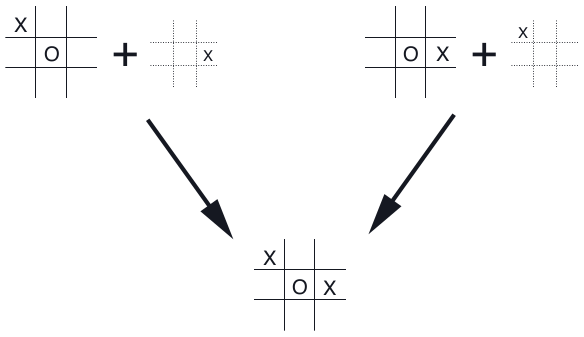
\includegraphics[width=0.8\textwidth]{img/afterstate_example.png}
    \caption{Two different state-action pairs that result in the same afterstate and therefore
        should have the same $Q$.}
    \label{fig:afterstate_example}
\end{figure}

A conventional action-value function would have to separately assess both pairs, whereas an
afterstate value function would immediately assess both equally.

\section{Summary}
In this chapter we introduced a new kind of learning method, temporal-difference (TD)
learning, and showed how it can be applied to the reinforcement learning problem.
As usual, we divided the overall problem into a prediction problem and a control problem.
TD methods are alternatives to Monte Carlo methods for solving the prediction problem.
In both cases, the extension to the control problem is via the idea of \myref{sec:gpi}{GPI}
that we abstracted from dynamic programming.
This is the idea that approximate policy and value functions should interact in such a way that
they both move toward their optimal values.
One of the two processes making up \myref{sec:gpi}{GPI}  drives the value function to accurately
predict returns for the current policy; this is the prediction problem.
The other process drives the policy to improve locally (e.g., to be $\epsilon$-greedy) with
respect to the current value function.
When the first process is based on experience, a complication arises concerning
maintaining sufficient exploration.
We can classify TD control methods according to whether they deal with this complication by
using an on-policy or off-policy approach.
\myref{sec:sarsa_on_policy_td_control}{Sarsa} is an on-policy method, and
\myref{sec:q_learning_off_policy_td_control}{Q-learning} is an off-policy method.
\myref{sec:expected_sarsa}{Expected Sarsa} is also an off-policy method as we present it here.
There is a third way in which TD methods can be extended to control which we did not include in
this chapter, called actor–critic methods.
These methods are covered in full in Chapter 13.
The methods presented in this chapter are today the most widely used reinforcement
learning methods.
This is probably due to their great simplicity: they can be applied online, with a minimal amount
of computation, to experience generated from interaction with an environment; they can be expressed
nearly completely by single equations that can be implemented with small computer programs.
In the next few chapters we extend these algorithms, making them slightly more complicated and
significantly more powerful.
All the new algorithms will retain the essence of those introduced here: they will be able
to process experience online, with relatively little computation, and they will be driven
by TD errors.
The special cases of TD methods introduced in the present chapter should rightly be called
one-step, tabular, model-free TD methods.
In the next two chapters we extend them to n-step forms (a link to Monte Carlo methods) and forms
that include a model of the environment (a link to planning and dynamic programming).
Then, in the second part of the book we extend them to various forms of function approximation
rather than tables (a link to deep learning and artificial neural networks).
Finally, in this chapter we have discussed TD methods entirely within the context of
reinforcement learning problems, but TD methods are actually more general than this.
They are general methods for learning to make long-term predictions about dynamical systems.
For example, TD methods may be relevant to predicting financial data, life spans, election outcomes,
weather patterns, animal behavior, demands on power stations, or customer purchases.
It was only when TD methods were analyzed as pure prediction methods, independent of their use in
reinforcement learning, that their theoretical properties first came to be well understood.
Even so, these other potential applications of TD learning methods have not yet been extensively
explored.


\chapter{$n$-step Bootstrapping}
\label{ch:n_step_bootstrapping}
Preferably \emph{bootstrapping} should be done over multiple steps, and that is what
these methods allow us to do.
The idea of $n$-step methods is usually used as an introduction to the algorithmic
idea of \emph{eligibility traces} (Chapter 12), which enable bootstrapping over
multiple time intervals simultaneously.

\section{$n$-step TD Prediction}
\label{sec:n_step_td_prediction}
\begin{figure}[h]
    \centering
    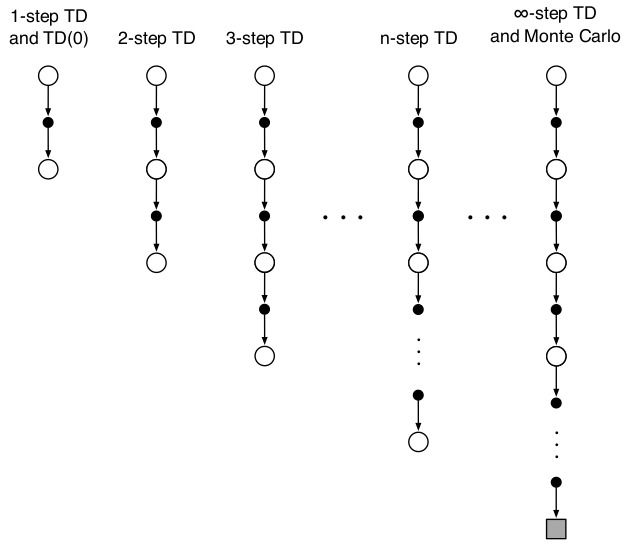
\includegraphics[width=0.7\textwidth]{img/n_step_td.png}
    \caption{The backup diagrams of $n$-step methods.
        These methods form a spectrum ranging from one-step TD methods to Monte
        Carlo methods.}
    \label{fig:7.1}
\end{figure}
\begin{myequation}{7.1}
    G_{t:t+n}\doteq
        R_{t+1}+\gamma R_{t+2}+\cdots+\gamma^{n-1}R_{t+n}+\gamma^nV_{t+n+1}(S_{t+n})
\end{myequation}
\begin{myequation}{7.2}
    V_{t+n}(S_t)\doteq V_{t+n-1}+\alpha\left(G_{t:t+n}-V_{t+n-1}(S_t)\right)
\end{myequation}

\begin{center}
    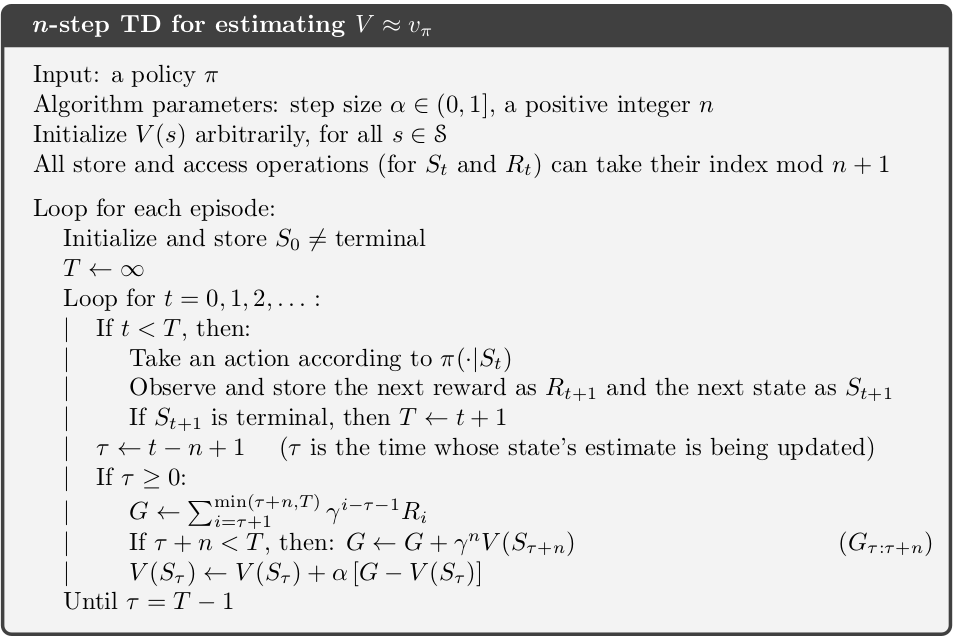
\includegraphics[width=\textwidth]{img/alg_n_step_td.png}
\end{center}

\section{$n$-step Sarsa}
\label{sec:n_step_sarsa}

\begin{myequation}{7.5}
    G_{t:t+n}\doteq\sum_{k=1}^{n}\gamma^{k-1}R_{t+k}+\gamma^nQ_{t+n-1}(S_{t+n},A_{t+n})\\
    Q_{t+n}(S_t,A_t)\doteq
        Q_{t+n-1}(S_t,A_t)+\alpha\left[G_{t:t+n}-Q_{t+n-1}(S_t,A_t)\right]
\end{myequation}

\begin{center}
    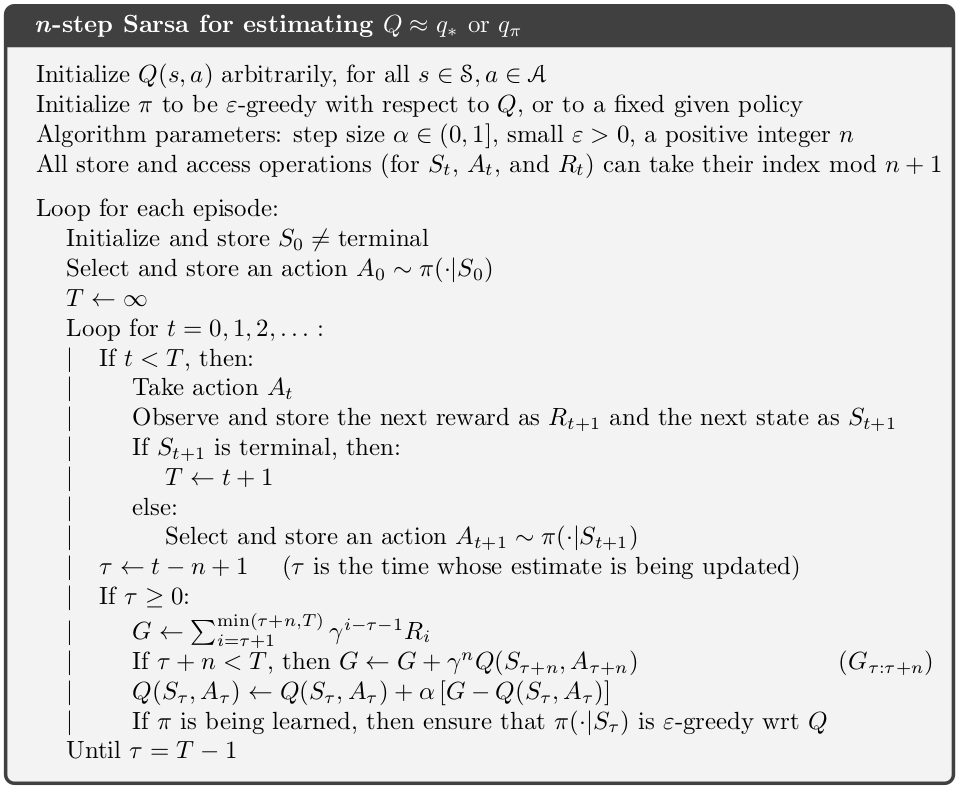
\includegraphics[width=\textwidth]{img/alg_n_step_sarsa.png}
\end{center}

\section{$n$-step Off-policy Learning}
\label{sec:n_step_off_policy_learning}
Other than the $\alpha$, the difference of gain and current value function value is weighted by
$\rho_{t:t+n-1}$.

\begin{myequation}{7.9}
    V_{t+n}(S_t)\doteq V_{t+n-1}(S_t)+\alpha \rho_{t:t+n-1}\left[G_{t:t+n}-V_{t+n-1}(S_t)\right]
\end{myequation}

\begin{myequation}{7.10}
    \rho_{t:h}\doteq\sum_{k=t}^{min(h,T-1)}\frac{\pi(A_k\mid S_k)}{b(A_k\mid S_k)}
\end{myequation}

\begin{myequation}{7.11}
    Q_{t+n}(S_t,A_t)\doteq
        Q_{t+n-1}(S_t,A_t)+\alpha \rho_{t+1:t+n}\left[G_{t:t+n}-Q_{t+n-1}(S_t,A_t)\right]
\end{myequation}

Note that here the \myref{t:importance_sampling_ratio}{importance sampling ratio} ($\rho$)
starts and ends one step later in comparison to the state-value function.
This is because we are not bothered with the current action taken, but rather only
looking at future actions.

\begin{center}
    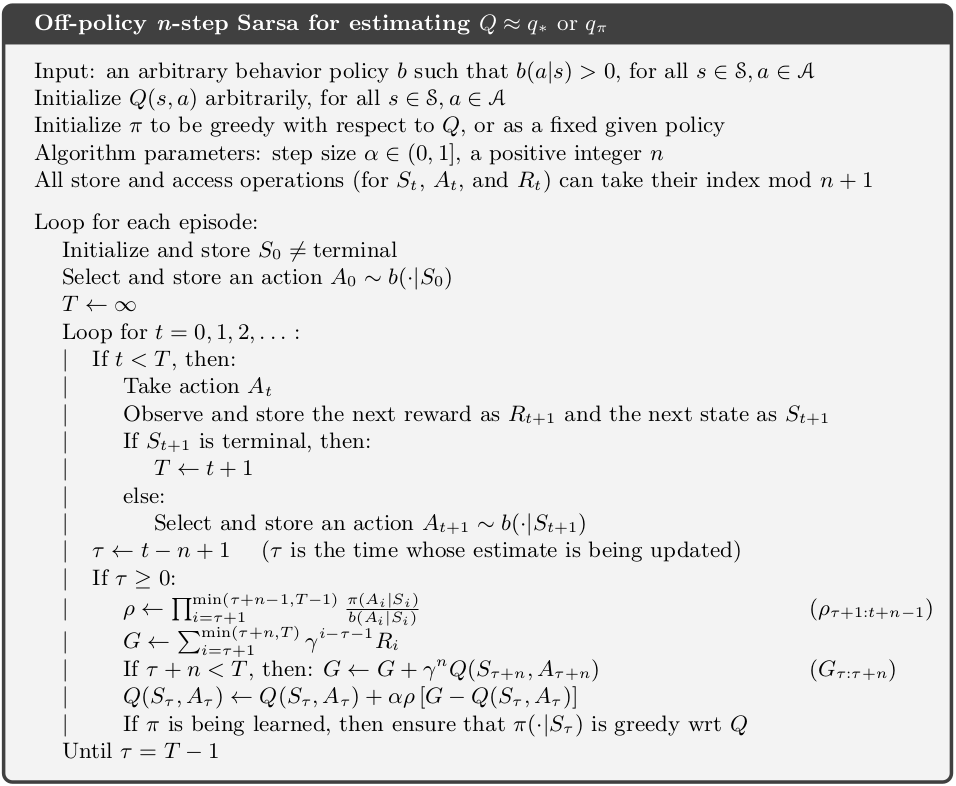
\includegraphics[width=\textwidth]{img/alg_off_policy_n_step_sarsa.png}
\end{center}


\section{*Per-decision Methods with Control Variates}
\label{sec:per_decision_methods_with_control_variates}
This approach takes a similar path to that in section
\ref{sec:per_decision_importance_sampling}.
\begin{myequation}{7.13}
    G_{t:h}\doteq\rho_t(R_{t+1}+\gamma G_{t+1:h})+(1-\rho_t)V_{h-1}(S_t) \\
    \rho_t\doteq \frac{\pi(A_t\mid S_t)}{b(A_t\mid S_t)} \hfill
    G_{h:h}\doteq V_{h-1}(S_h)
\end{myequation}

The $(1-\rho_t)V_{h-1}(S_t)$ term is called the \emph{control variate}\label{t:control_variate}.
It is used to take the value of the resulting state as the approximation of the gain following it.
This term has an effect on $G_{t:h}$ only when $b$ takes actions that are improbable in $pi$.

For a conventional n-step method, the learning rule to use in conjunction with (\ref{eq:7.13})
is the n-step TD update (\ref{eq:7.2}), which has no explicit importance sampling ratios other
than those embedded in the return.

\begin{myequation}{7.14}
    G_{t:h}\doteq
        R_{t+1}+\gamma\rho_{t+1}(G_{t+1:h}-Q_{h-1}(S_{t+1},A_{t+1}))
        +\gamma\bar{V}_{h-1}(S_t+1)\\
        \bar{V}_t(s)\doteq \sum_a\pi(a\mid s)Q_t(s,a) \\
        h<T\Rightarrow G_{h:h}\doteq Q_{h-1}(S_h,A_h)\\
        h\geq T\Rightarrow G_{T-1:h}\doteq R_T
\end{myequation}

\section{Off-policy Learning Without Importance Sampling: The $n$-step Tree Backup Algorithm}
\label{sec:off_policy_learning_without_importance_sampling}

\begin{wrapfigure}[14]{l}{0.2\textwidth}
    \centering
    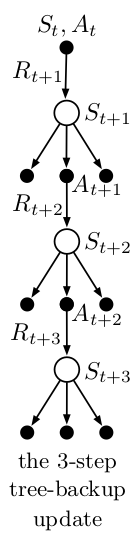
\includegraphics[width=0.2\textwidth]{img/n_step_tree_backup_diagram.png}
\end{wrapfigure}
This algorithm takes into consideration actions not taken.
We go down the taken action to calculate the $G$ but add to it the possibility of taking
and the value of actions \textbf{not taken}.
The last node's gain is calculated just like for \myref{sec:expected_sarsa}{expected sarsa}.
\begin{myequation}{7.15}
    G_{t:t+1}\doteq R_{t+1}+\gamma\sum_{a}\pi(a\mid S_{t+1})Q_t(S_{t+1},a)\\
    \begin{aligned}
        G_{t:t+2}\doteq
        &R_{t+1}+\gamma\sum_{a\neq A_{t+1}}\pi(a\mid S_{t+1})Q_{t+1}(S_{t+1},a)\\
        &+\gamma\pi(A_{t+1}\mid S_{t+1})G_{t+1:t+2}
    \end{aligned}
\end{myequation}
Generalizing to:
\begin{myequation}{7.16}
    \begin{aligned}
        G_{t:t+n}\doteq
        &R_{t+1}+\gamma\sum_{a\neq A_{t+1}}\pi(a\mid S_{t+1})Q_{t+1}(S_{t+1},a)\\
        &+\gamma\pi(A_{t+1}\mid S_{t+1})G_{t+1:t+n}
    \end{aligned} \\
    G_{T-1:t+n}\doteq R_T
\end{myequation}
The update rule is the same as in the $n$-step Sarsa:
\begin{equation*}
    Q_{t+n}\doteq Q_{t+n-1}(S_t,A_t)+\alpha\left[G_{t:t+n}-Q_{t+n-1}(S_t,A_t)\right]
\end{equation*}

\begin{center}
    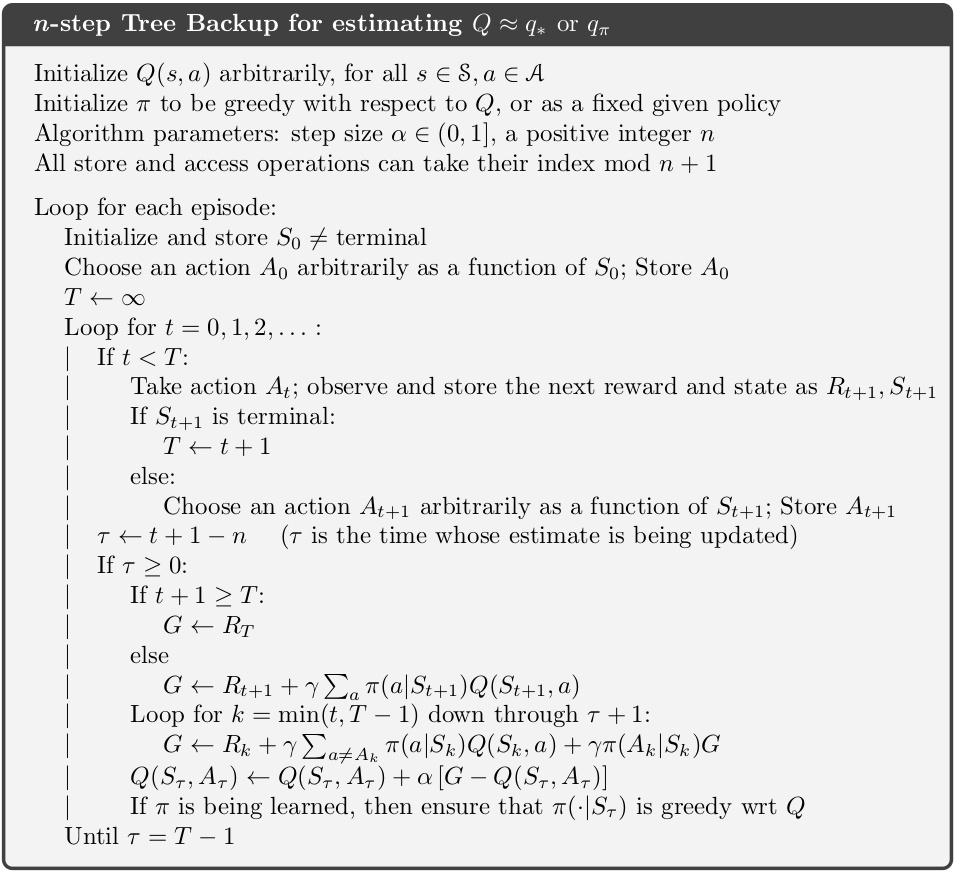
\includegraphics[width=\textwidth]{img/alg_n_step_tree_backup.png}
\end{center}

\section{*A Unifying Algorithm: $n$-step $Q(\sigma)$}
\label{sec:a_unifying_algorithm_n_step_q_sigma}

\begin{center}
    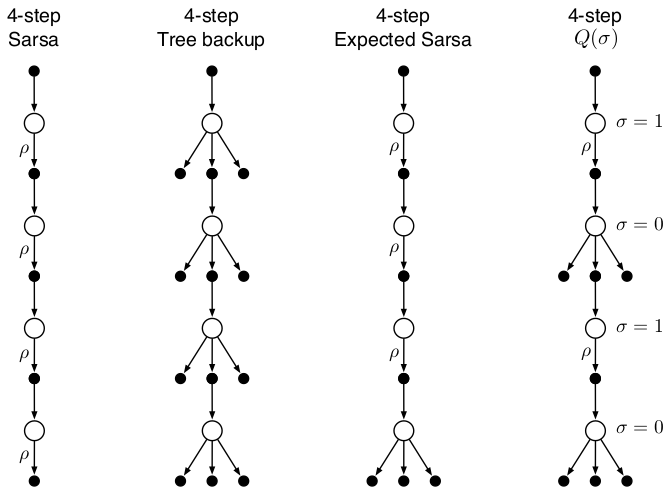
\includegraphics[width=\textwidth]{img/n_step_q_sigma_backup_diagram.png}
\end{center}

Depending on the \emph{random} variable $\sigma\in[0,1]$ the algorithm either samples
with \myref{t:importance_sampling_ratio}{importance sampling} or
calculates via expectations and $\pi$.
$\sigma$ can be a function of $t$, $s$, $(s,a)$,...

\begin{myequation}{7.17}
    \begin{aligned}
        G_{t:h}\doteq
            R_{t+1}+&\gamma\left(
                \sigma_{t+1}\rho_{t+1}
                +(1-\sigma_{t+1})\pi(A_{t+1}\mid S_{t+1})\right)
            \left(G_{t+1:h}-Q_{h-1}(S_{t+1},A_{t+1})\right)\\
            +&\gamma\bar{V}_{h-1}(S_{t+1})
    \end{aligned} \\
    \begin{aligned}
        &G_{h:h}\doteq Q_{h-1}(S_h,A_h), &h<T \\
        &G_{T-1:h}\doteq R_T, &h==T
    \end{aligned}
\end{myequation}
The update rule is the same as in the $n$-step Sarsa:
\begin{equation*}
    Q_{t+n}\doteq Q_{t+n-1}(S_t,A_t)+\alpha\left[G_{t:t+n}-Q_{t+n-1}(S_t,A_t)\right]
\end{equation*}

\begin{center}
    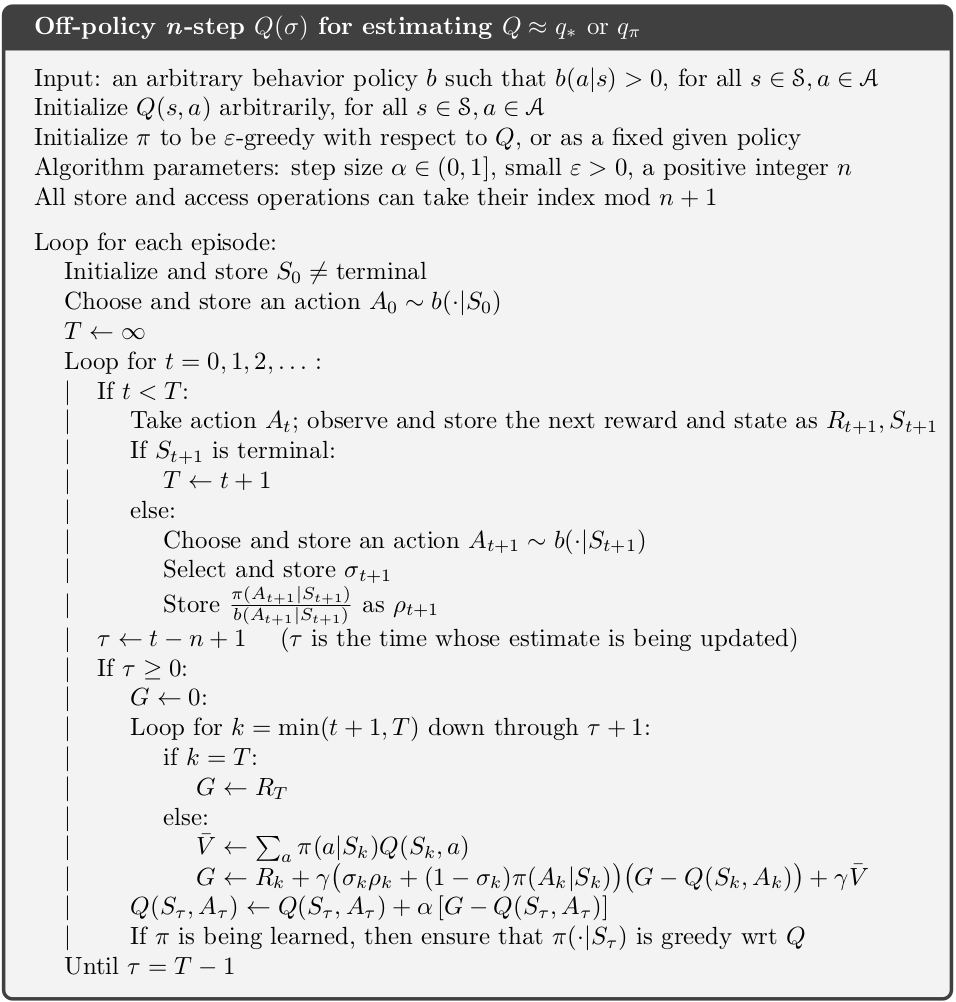
\includegraphics[width=\textwidth]{img/alg_n_step_q_sigma.png}
\end{center}

\section{Summary}
\label{sec:nsb-summary}
In this chapter we have developed a range of temporal-difference learning methods that lie
in between the one-step TD methods of the previous chapter and the Monte Carlo methods
of the chapter before.
Methods that involve an intermediate amount of bootstrapping are important because they will
typically perform better than either extreme.
Our focus in this chapter has been on $n$-step methods, which look ahead to the next $n$ rewards,
states, and actions.
All $n$-step methods involve a delay of $n$ timesteps before updating, as only then are all the
required future events known.
A further drawback is that they involve more computation per timestep than previous methods.
Compared to one-step methods, $n$-step methods also require more memory to record the states,
actions, rewards, and sometimes other variables over the last $n$ time steps.
Eventually, in Chapter 12, we will see how multi-step TD methods can be implemented with
minimal memory and computational complexity using eligibility traces, but there will always be some
additional computation beyond one-step methods.
Such costs can be well worth paying to escape the tyranny of the single time step.
Although $n$-step methods are more complex than those using eligibility traces, they have
the great benefit of being conceptually clear.
We have sought to take advantage of this by developing two approaches to off-policy learning in
the $n$-step case.
One, based on importance sampling is conceptually simple but can be of high variance.
If the target and behavior policies are very different it probably needs some new algorithmic
ideas before it can be efficient and practical.
The other, based on tree-backup updates, is the natural extension of Q-learning to the multi-step
case with stochastic target policies.
It involves no importance sampling but, again if the target and behavior policies are substantially
different, the bootstrapping may span only a few steps even if $n$ is large.


\chapter{Planning and Learning with Tabular Methods}
\label{ch:planning_and_learning_with_tabular_methods}
Model-based methods rely on \emph{planning} as their primary component, while model-free methods
primarily rely on \emph{learning}.


%%%%% SECTION
\section{Models and Planning}
\label{sec:models_and_planning}
\emph{Distribution models}\label{t:distribution_model} produce a description of all possibilities
after a $(s,a)$ pair and their probabilities.
\emph{Sample models}\label{t:sample_model} produce just one of the possibilities after a $(s,a)$
pair, sampled according to the probabilities.
Obviously distribution models are more useful, and if needed they can be used to create samples
and have the output of the sample models.
The opposite is not possible.
The model is used to \emph{simulate} the environment and produce \emph{simulated experience}.
\emph{Planning}\label{t:planning} is a computational process that takes a model as input and
produces or improves a policy for interacting with the modeled environment:
\begin{center}
    
\includegraphics[scale=0.5]{img/model_planning_policy.png}
\end{center}
Two distinct approaches to planning:
\begin{itemize}
    \item \emph{State-space planning}\label{t:state_space_planning}:
        a search through the state space for an optimal policy or an optimal path to a goal.
        Value functions are computed for states or state-action pairs and actions cause
        transitions from state to state.
    \item \emph{Plan-space planning}\label{t:plan_space_planning}:
        a search through the space of plans.
        Operators transform one plan into another, and value functions, if any, are defined over
        the space of plans.
        These methods are difficult to apply efficiently to the stochastic sequential decision
        problems that are the focus in reinforcement learning, and we do not consider them further.
\end{itemize}
All \myref{t:state_space_planning}{state-space planning methods} share a common structure:
\begin{enumerate}
    \item They all involve computing value functions as a key intermediate step to improving the
        policy.
    \item They compute value functions by updates or backup operations applied to simulated
        experience.
\end{enumerate}
\begin{center}
    
\includegraphics[width=\textwidth]{img/structure_state_space_planning.png}
\end{center}

Planning uses simulated experience generated by a model, learning methods use real experience
generated by the environment.

\begin{center}
    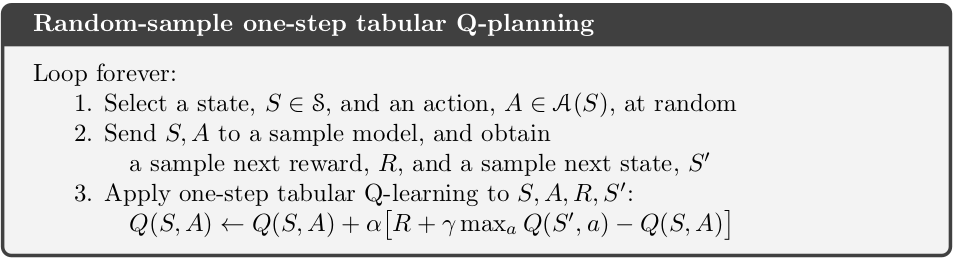
\includegraphics[width=\textwidth]{img/alg_random_sample_one_step_tabular_q_learning.png}
\end{center}


%%%%% SECTION
\section{Dyna: Integrated Planning, Acting, and Learning}
\label{sec:dyna_integrated_planning_acting_and_learning}
\begin{wrapfigure}{r}{0.4\textwidth}
    \centering
    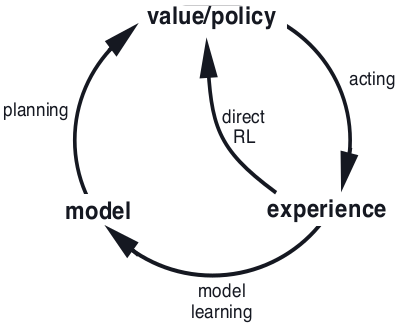
\includegraphics[width=0.4\textwidth]{img/dyna_q_diagram.png}
\end{wrapfigure}
Within a planning agent, there are at least two roles for real experience: it can be
used to improve the model (to make it more accurately match the real environment)
and it can be used to directly improve the value function and policy using the kinds of
reinforcement learning methods we have discussed in previous chapters.
The former we call \emph{model-learning}\label{t:model_learning}, and the latter we call
\emph{direct reinforcement learning} (direct RL).
Dyna-Q includes all of the processes shown in the diagram above - planning, acting,
model-learning, and direct RL - all occurring continually.
\begin{itemize}
    \item planning: one-step tabular Q-planning
    \item direct RL: one-step tabular Q-learning
    \item model learning: stores transitions deterministically in the table
\end{itemize}
During planning the random sampling from the model is done only for $(s,a)$ that have been
experienced.

\begin{figure}[h]
    \centering
    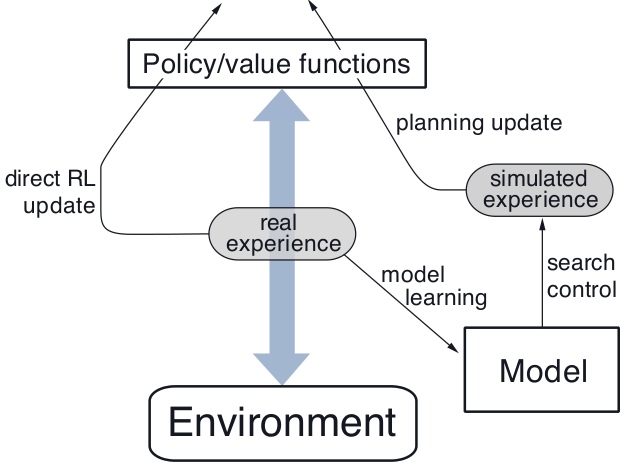
\includegraphics[width=0.8\textwidth]{img/dyna_architecture.png}
    \caption{The general Dyna Architecture.
        Real experience, passing back and forth between the environment and the policy,
        affects policy and value functions in much the same way as does simulated experience
        generated by the model of the environment.}
    \label{fig:dyna_architecture}
\end{figure}

\begin{center}
    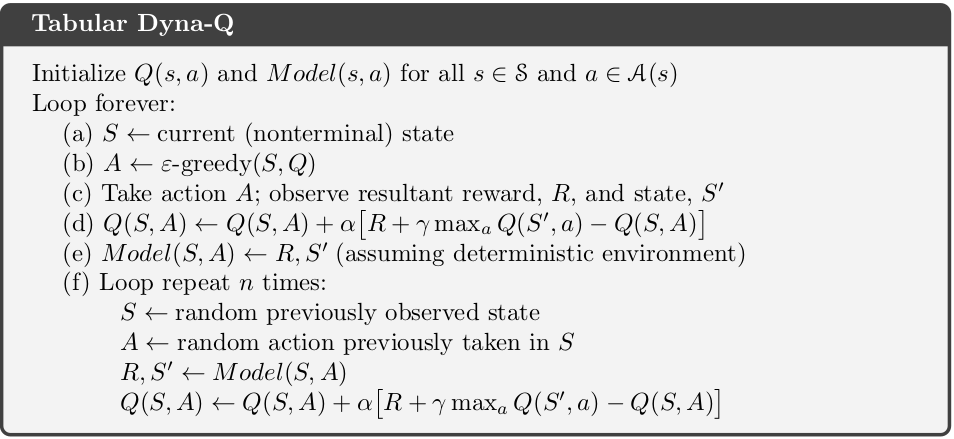
\includegraphics[width=\textwidth]{img/alg_tabular_dyna_q.png}
\end{center}


%%%%% SECTION
\section{When the Model Is Wrong}
\label{sec:when_the_model_is_wrong}
Models may be incorrect because the environment is stochastic and only a limited number of samples
have been observed, or because the model was learned using function approximation that
has generalized imperfectly, or simply because the environment has changed and its new
behavior has not yet been observed.
The suboptimal policy computed by planning quickly leads to the discovery and correction of the
modeling error.
This tends to happen when the model is optimistic in the sense of predicting greater reward or
better state transitions than are actually possible.
The planned policy attempts to exploit these opportunities and in doing so discovers that they do
not exist.

The Dyna-Q+ agent uses a heruistic where it tracks the last time a particular $(s,a)$ pair has
been last tried in a real interaction with the environment.
The more time passes the greater the possibility that the dynamics of the environment under such a
$(s,a)$ pair have changed.
To stimulate the agent to take these exploratory steps a special \emph{bonus reward} is given in
simulated experiences involving these actions.
In particular, if the modeled reward for a transition is $r$, and the transition has not been tried
in $\tau$ time steps, then planning updates are done as if that transition produces a reward
of $r+\kappa\sqrt{\tau}$, for some small $\kappa$.


%%%%% SECTION
\section{Prioritized Sweeping}
\label{sec:prioritized_sweeping}
Pick transitions to learn from using a kind of priority.
Realize that some transitions will not provide any added knowledge, while other might.
It would be good to work \emph{backwards} from goal states, but this notion can be extended to
working back from any state whose value has changed.
One can work backward from arbitrary states that have changed in value, either performing
useful updates or terminating the propagation.
This general idea might be termed backward focusing of planning computations.
A queue is maintained of every state–action pair whose estimated value would change
nontrivially if updated, prioritized by the size of the change.
When the top pair in the queue is updated, the effect on each of its predecessor pairs is
computed.
If the effect is greater than some small threshold, then the pair is inserted in the queue
with the new priority (if there is a previous entry of the pair in the queue, then insertion
results in only the higher priority entry remaining in the queue).
Priority is assigned using \myref{eq:6.8}{td error for Q-learning}.

\begin{center}
    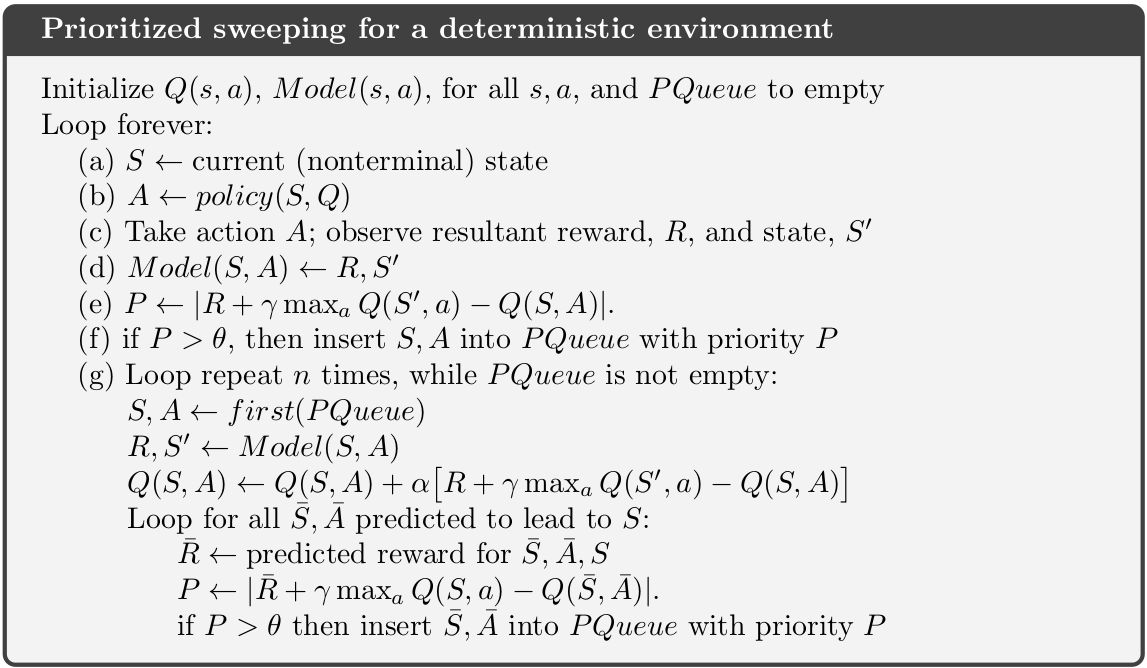
\includegraphics[width=\textwidth]{img/prioritized_sweeping.png}
\end{center}
(g) - backpropagate the update to previous states as long as $\delta$ is over $\theta$.


%%%%% SECTION
\section{Expected vs. Sample Updates}
\label{sc:expected_vs_sample_updates}



\end{document}
